\section{Measurement}\label{sec:measurement}
This section is a description on how the \etaDal \ was simulated and reconstructed for this CLAS12 proposal.
\subsection{Simulation and Reconstruction}
To simulate the reaction in Eq.~\ref{eq:etaP}, the program PLUTO++~\cite{PLUTO} was utilize for its ability to simulate the decays of those according to QED, Vector Meson Dominance or a user defined TFF. For reconstruction of the desired topologies, the CLAS12 FASTMC~\cite{fastmc} was used, in which $\sim 5\cdot10^8$ events were generated for \etaPDal \ and then simulated with FASTMC at 75\% torus field. The efficiency for all detectors are assumed to be 100\% and only the geometric acceptance is considered for this proposal. Therefore the numbers that will be quoted in this proposal will be only an upper limit. An extra FASTMC simulation was performed for the torus field setting of 100\% to show the effects of the magnetic field on the lepton acceptance. 
%The EC efficiency  was calculated by comparing GEMC (GEANT4) simulations with FASTMC. This EC efficiency was also calculated with the g12 data set and was identical to the comparison of the two simulation methods.
 \newline
\indent The production of \etaTP \ was weighted by photo-production differential cross-sections, $\frac{d\sigma}{d\Omega}(v,\cos\theta_{cm})$, published in~\cite{Williams}, and $Q^2$. Where $v$ is the virtual photon energy, $\cos\theta_{cm}$ is the production angle in the center-of-mass frame of the system and $Q^2$, the production virtual photon, is defined as $-(k-k')^2$. This was done to achieve a quasi realistic model of the production. The \epemT \  decay spectrum, of each meson, was weighted via the VMD model (including QED predictions). Another simulation was performed using a flat $M(\epem)$ distribution (No QED, No VMD) to analyze any effects of the model on the \epemT acceptance. The analysis showed that the acceptance, in $M(\epem)$, was independent of the decay model, see Fig.\ref{fig:VMDaccepted} and Fig.\ref{fig:FLATaccepted}.
\subsubsection{Trigger Requirements}
The standard CLAS12 electron trigger (HTCC(Nphe>2) * [ (PCAL+EC)>1.0 GeV ] is sufficient for this types of analysis. The rate for hadron production in electro-production where the scattered electron is left undetected is $\sim 140\,\rm{kHz}$~\cite{Sargsyan}. This rate needs to be scaled down by the ratio of hardon production cross-section to \etaTP \ production cross-section, see Eq.~\ref{XsecR} in Sec.~\ref{sec:yield}. This ratio was calculated $\sim\frac{1}{200}$, which leads to an overall rate of 0.7~kHz, while the expected data acquisition (DAQ) readout rate is 10~kHz.
\subsubsection{Detection of \epemT Events} 
Electron/positron ID will include responses from the HTCC, PCAL and EC calorimeters. The energy information of the PCAL and the inner and outer parts of EC will be used to compare the total energy deposition with the momentum measured in the DC ($\alpha*(\mathrm{E_{Pcal}} + \mathrm{E_{ECin}}+ \mathrm{E_{ECout}}) \sim \mathrm{P_{DC}}$), where $\alpha$ is a scaling factor.
\subsubsection{Particle Identification}
The $\etaP$ meson have pion decay modes, which are orders of magnitude greater than the Dalitz decay. For example, the ratio $\Gamma_{\pi^+\pi^-\gamma} / \Gamma_{e^+e^- \gamma} $ is $ 6.2\cdot 10^2$. 
Electrons/positrons will be identified by using the information from the detectors described above. The expected $e^\pm/\pi^\pm$ rejection factor for single particles (p<4.9~GeV) is $10^3$ for the HTCC, while the PCAL+EC can provide an additional factor of $10^2$. Combining both methods yields a $e^\pm/\pi^\pm$ rejection factor of $10^5$ which results in a $e^+e^-/\pi^+\pi^-$ rejection factor of $10^{10}$. Therefore, the amount of $\pi^+\pi^-$ background in the $M(\epem)$ spectrum will be $\approx 6.2\cdot 10^2/10^{10} = 6.2\cdot10^{-8}$. A detailed explanation of particle identification for \epemT \ pairs can be found in~\cite{clas.proposal.jpsi}.
\subsubsection{Acceptance}\label{sec.reconstruction}
An inclusive reconstruction scheme
\begin{align}
ep\to e'p \etaP \rightarrow p e^+ \gamma e^- (e^-)
\end{align}
where a proton, a photon, a positron and one electron of unknown source is detected. It will be determined from kinematics which electron corresponds to the beam scattered electron or the Dalitz produced electron. 
\todo{Add daniels plots}
The acceptance was calculated by dividing the accepted events by the generated events, per $M(\epem)$ bin. The $\etaP$ Dalitz decay acceptance using the VMD as a decay model can be seen in Fig.\ref{fig:VMDaccepted}, while the acceptance using a flat \epemT \ mass distribution can be seen in Fig.~\ref{fig:FLATaccepted}. A comparison of these two figures shows a model independent \epemT \ acceptance. 
%\begin{figure}[h!]\begin{center}
%		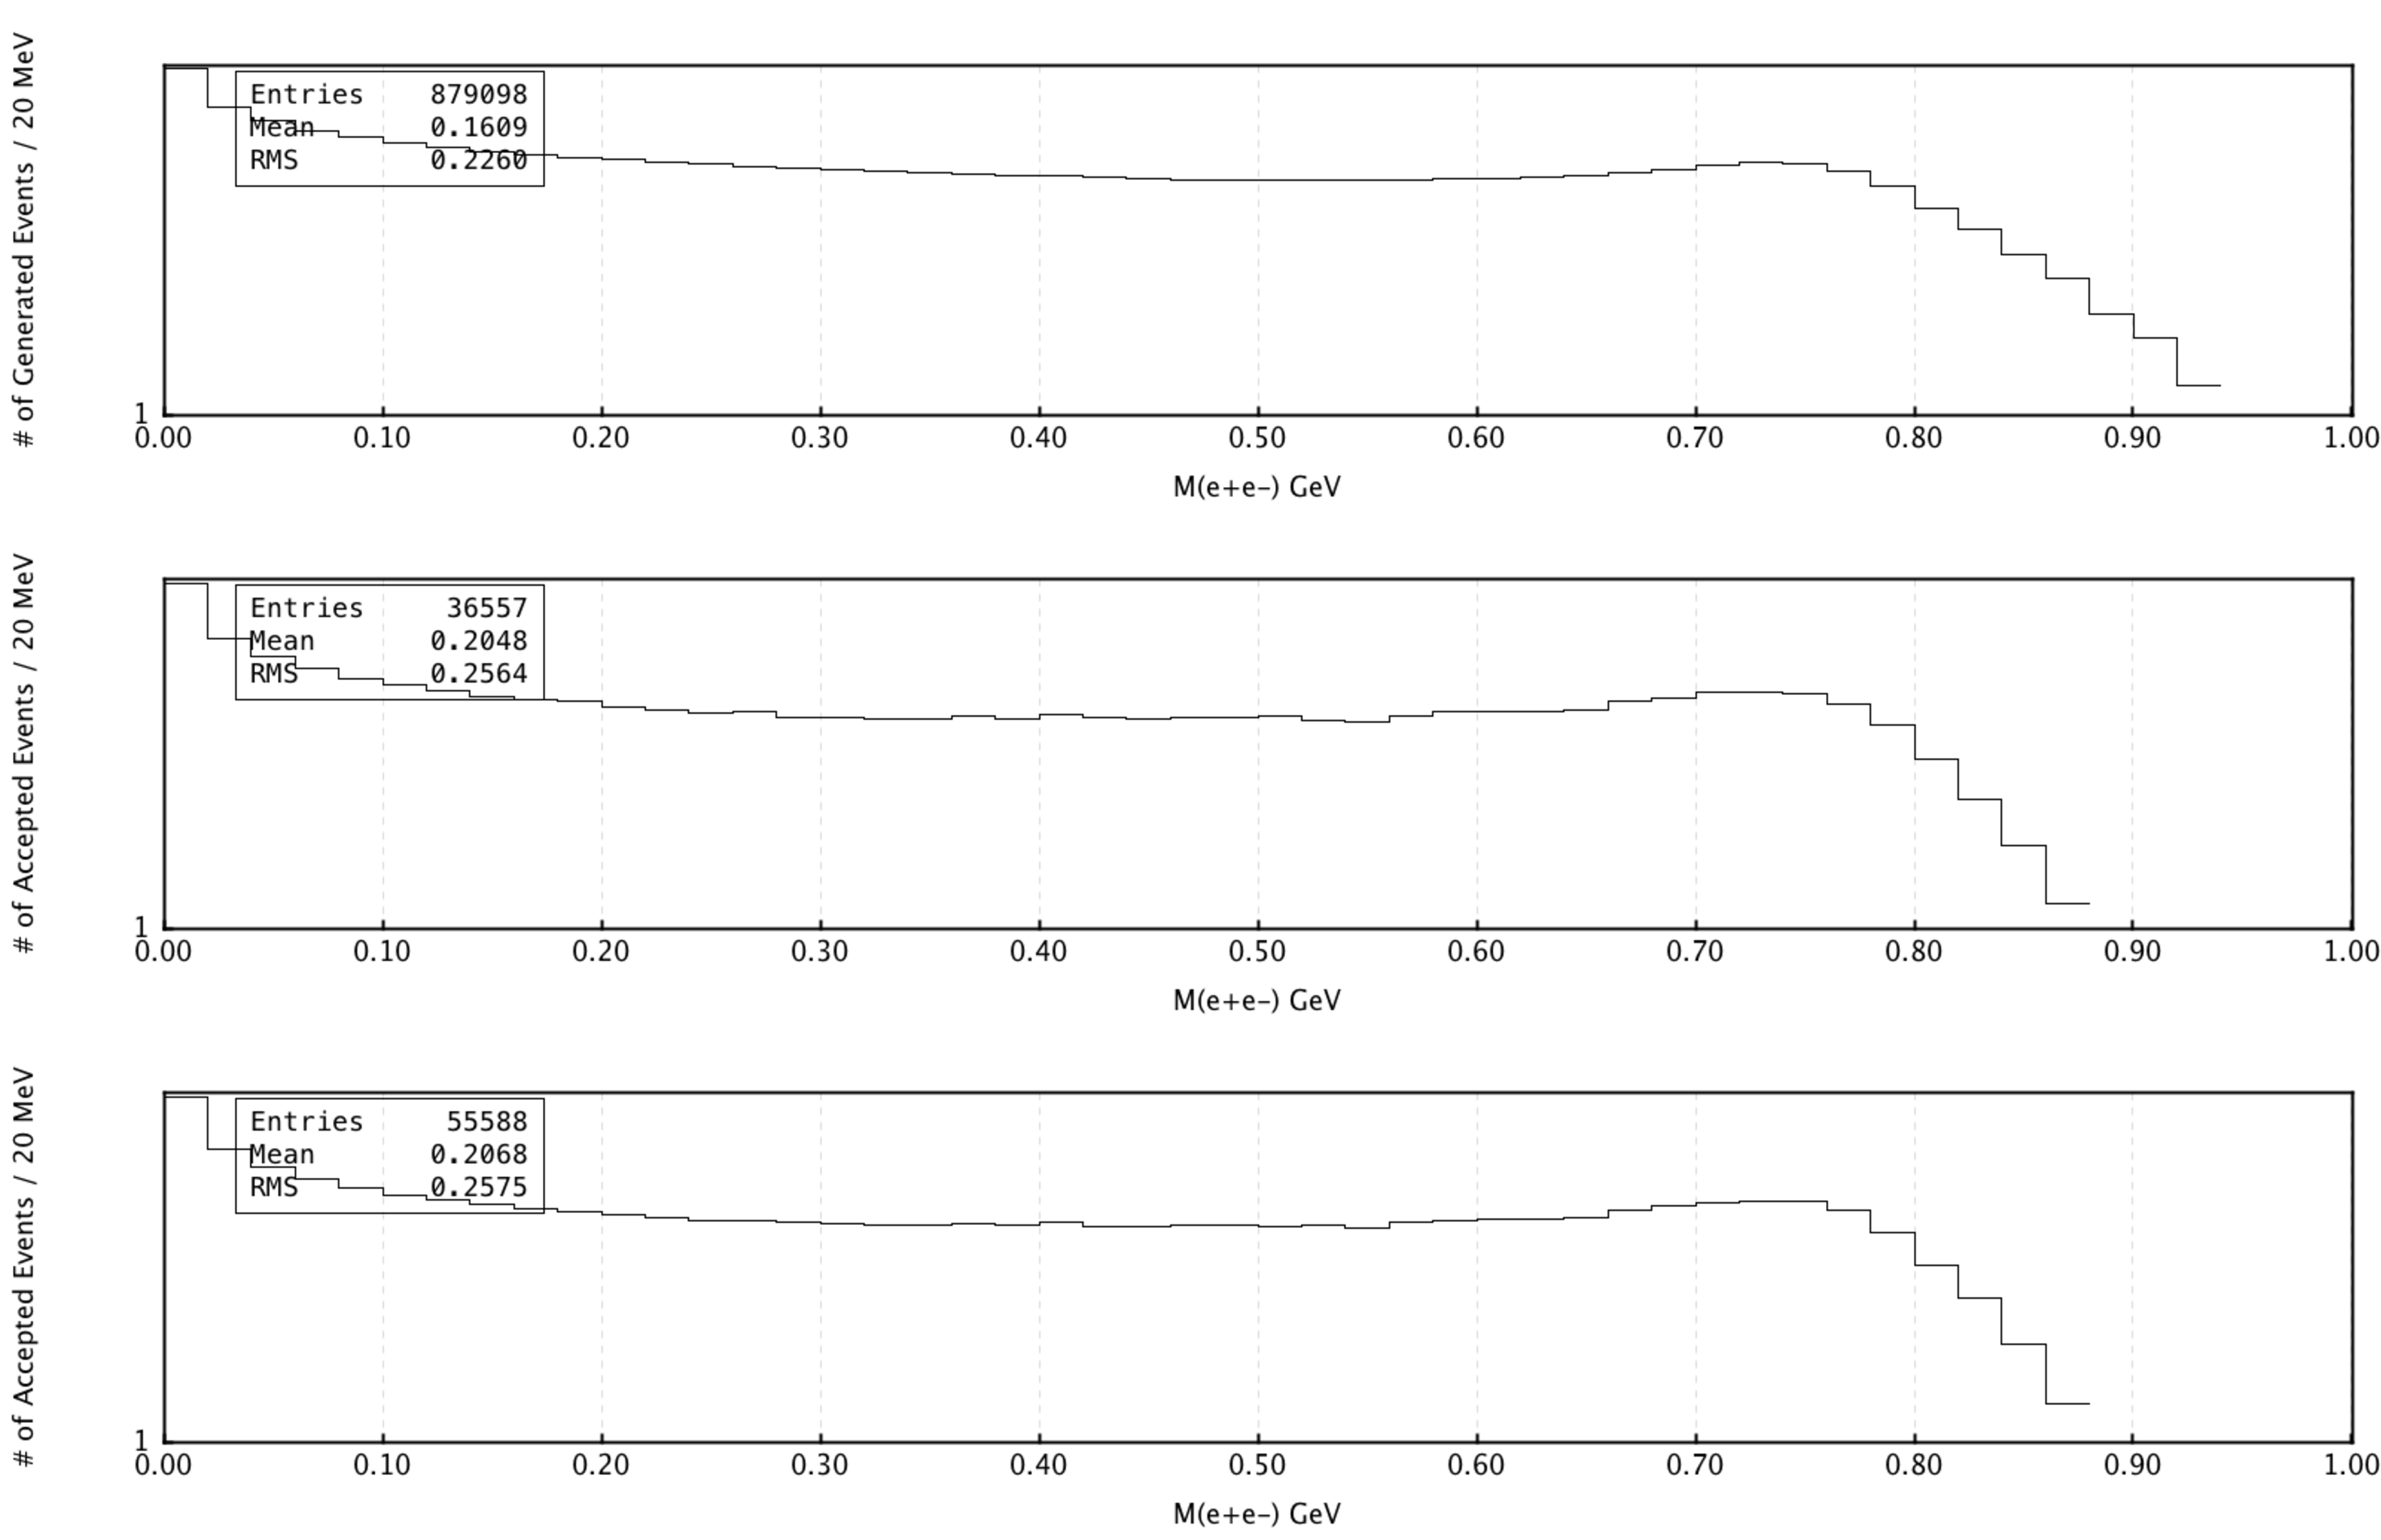
\includegraphics[width=\figwidth,height=2.6\qfigheight]{\grpath/counts/75_TORUS/VMD/VMD_Generated_Accepted.pdf}
%		\caption[Generated and Accepted counts, as a function of $M(\epem)$]{\label{fig:VMD}{Generated events (Top), accepted events for an exclusive (Middle), inclusive(Bottom) reconstruction schemes as a function of $M(\epem)$. In all panels a VMD decay model was employed}}
%\end{center}\end{figure}
%\begin{figure}[h!]\begin{center}
%			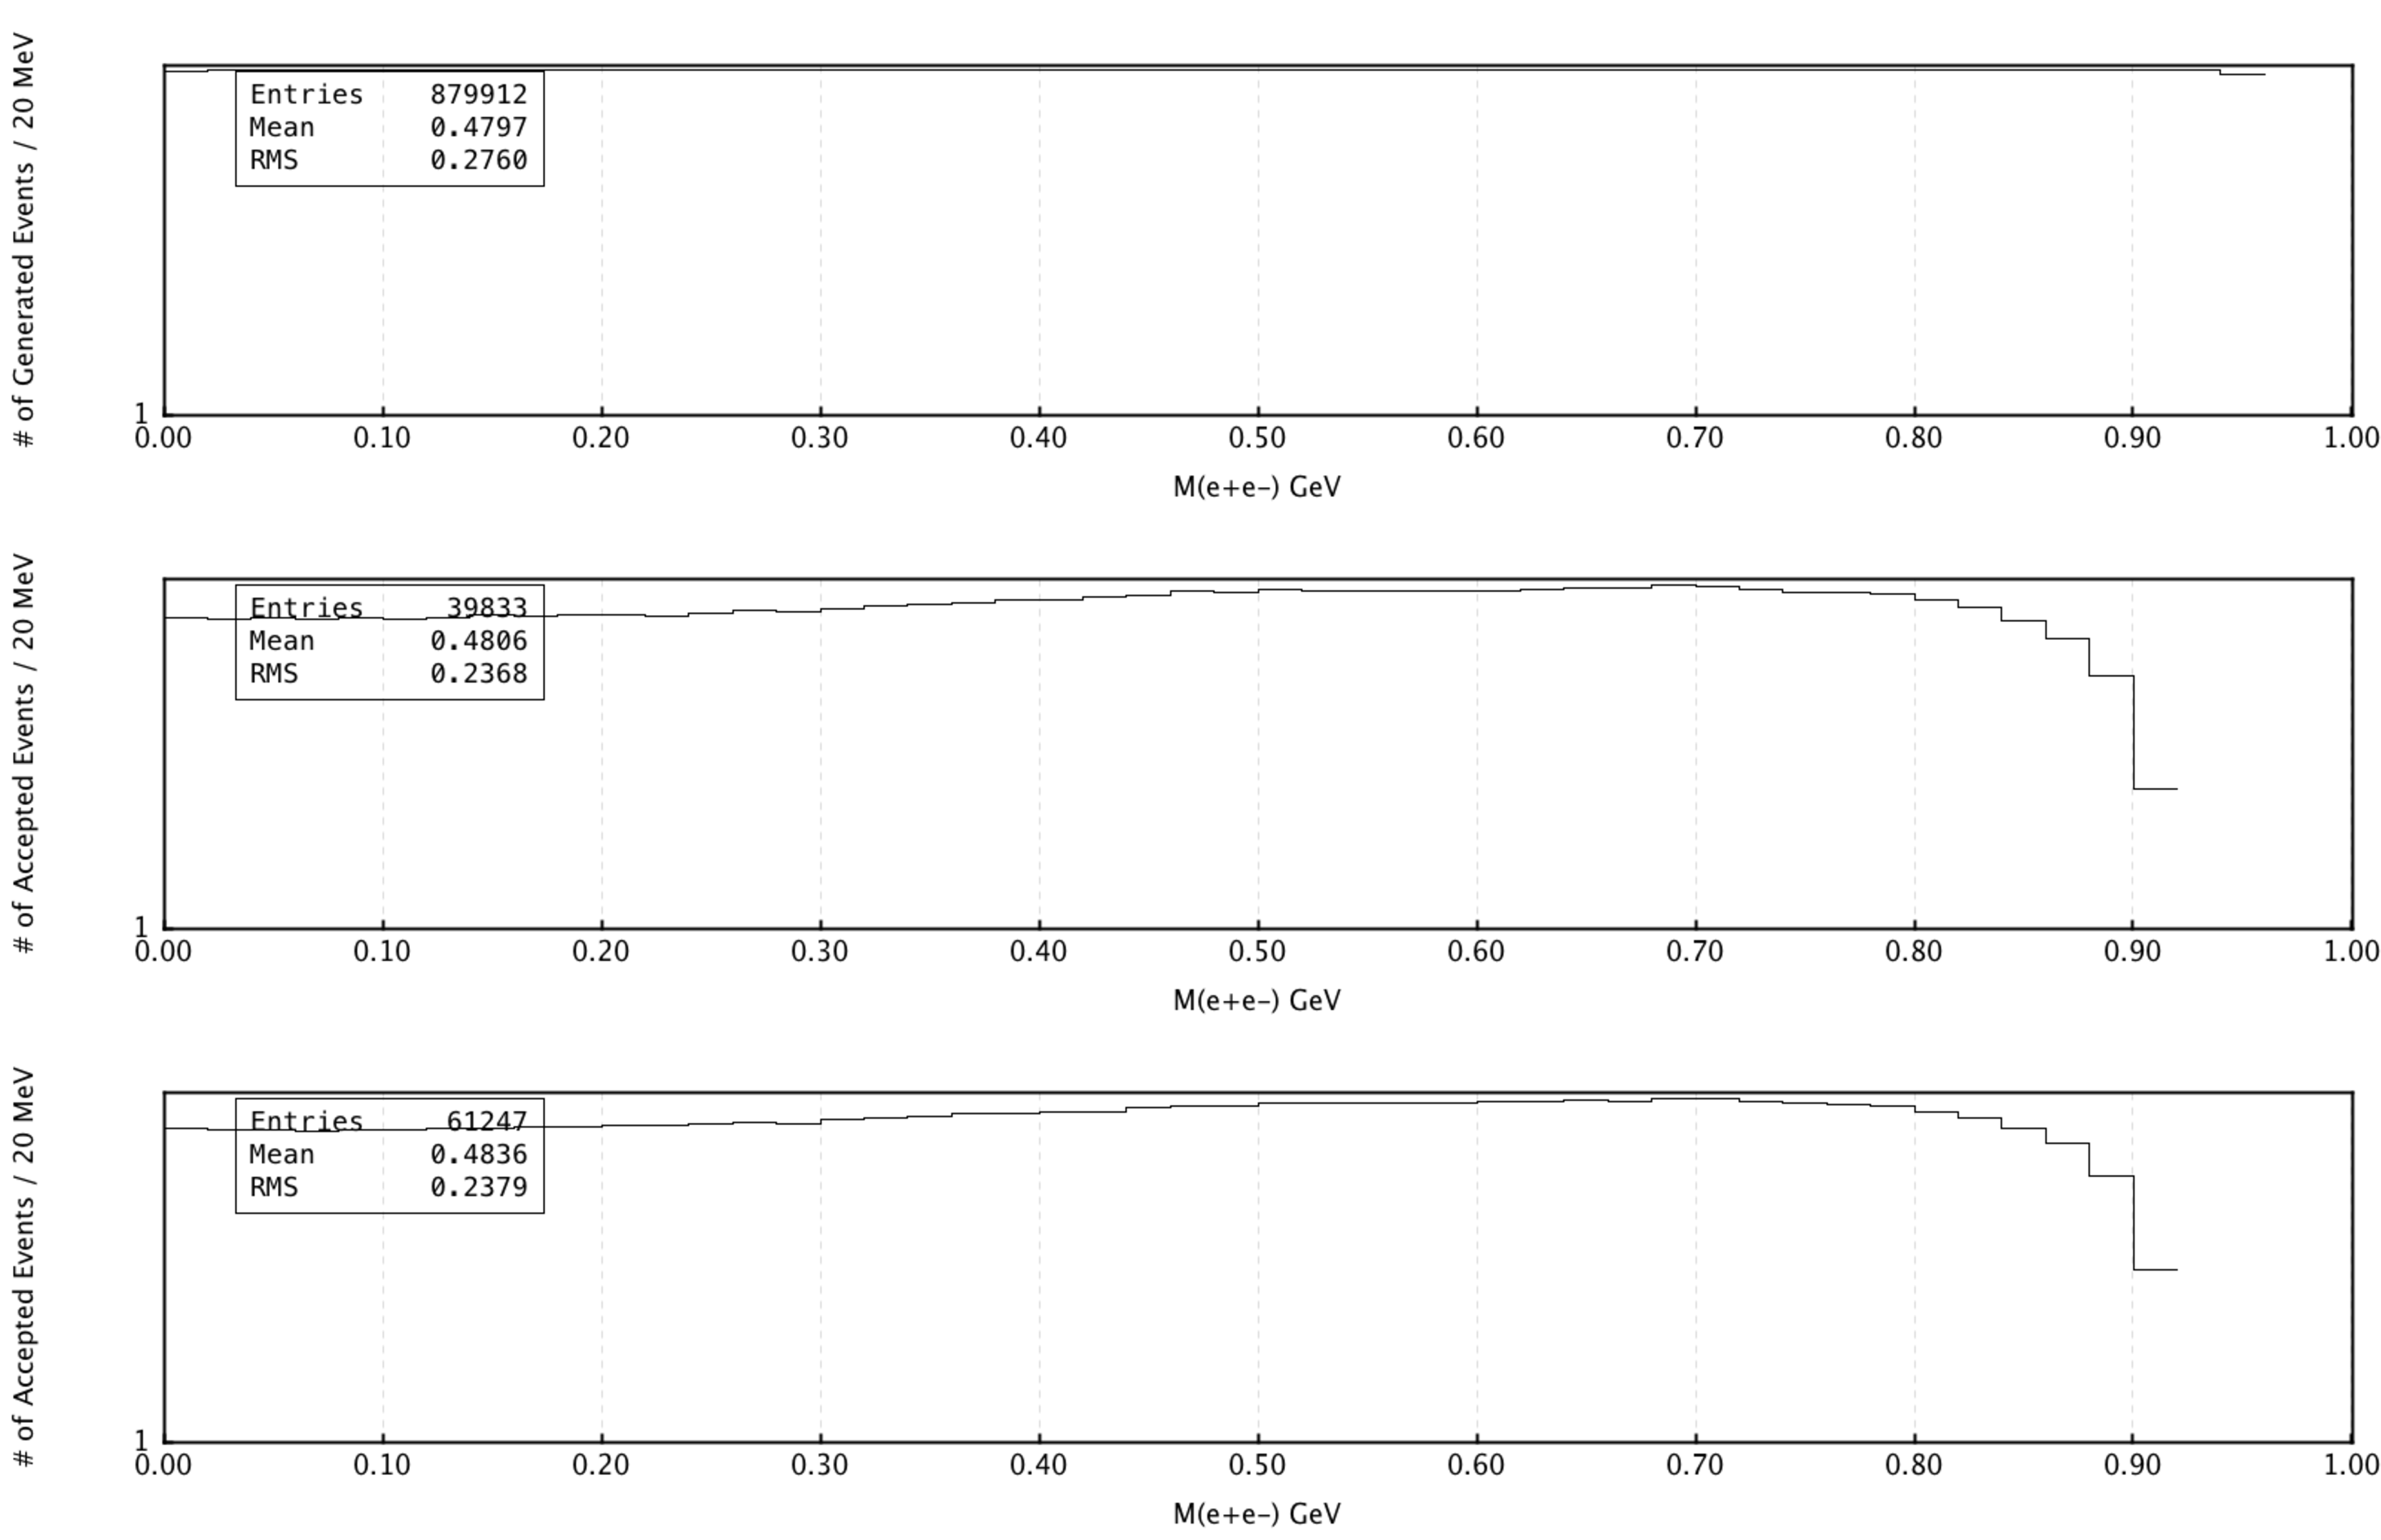
\includegraphics[width=\figwidth,height=2.6\qfigheight]{\grpath/counts/75_TORUS/FLAT/FLAT_Generated_Accepted.pdf}
%			\caption[Generated and Accepted counts, as a function of $M(\epem)$]{\label{fig:FLAT}{Generated events (Top), accepted events for an exclusive (Middle), inclusive(Bottom) reconstruction schemes as a function of $M(\epem)$. In all panels a Flat \epemT \ decay model was employed}}
%\end{center}\end{figure}
\FloatBarrier

\begin{figure}[h!]\begin{center}
		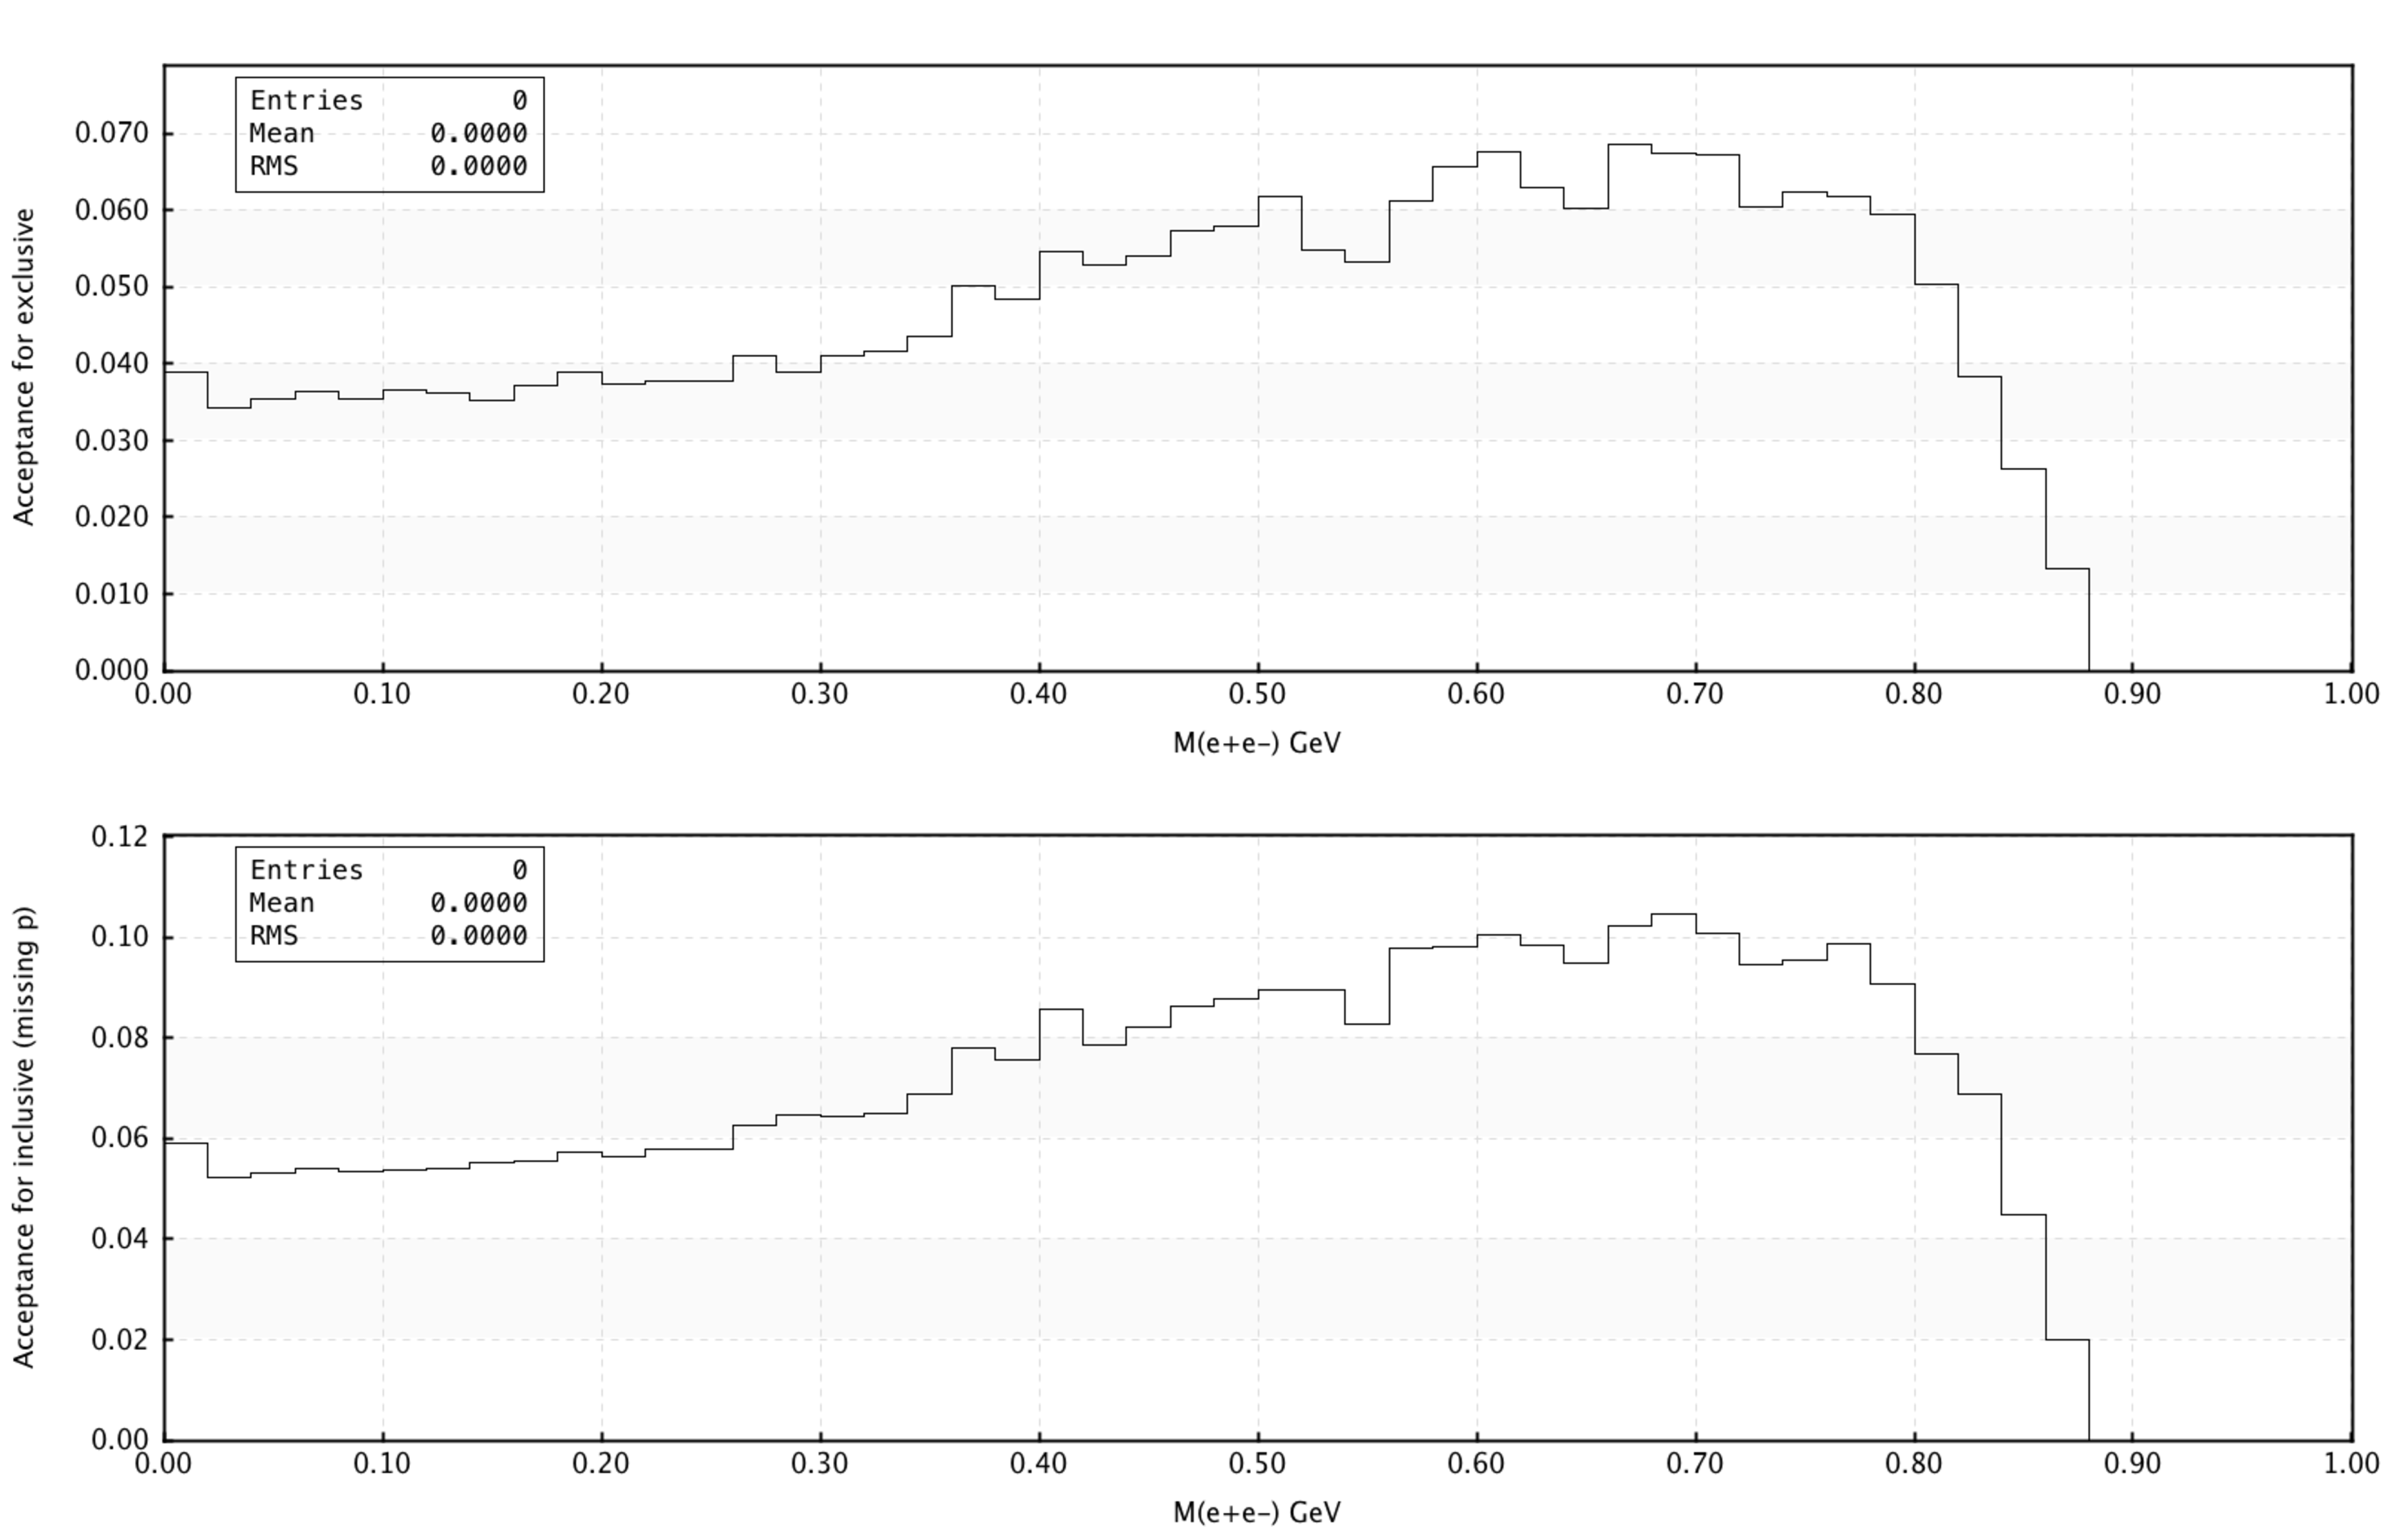
\includegraphics[width=\figwidth,height=1.2\qfigheight]{\grpath/counts/75_TORUS/VMD/VMD_Acceptance.pdf}
		\caption[Acceptance, as a function of $M(\epem)$]{\label{fig:VMDaccepted}{Acceptance using a VMD decay model, as a function of $M(\epem)$ for the exclusive (Top) and inclusive reconstruction scheme(Bottom). }}
\end{center}\end{figure}

 \begin{figure}[h!]\begin{center}
 		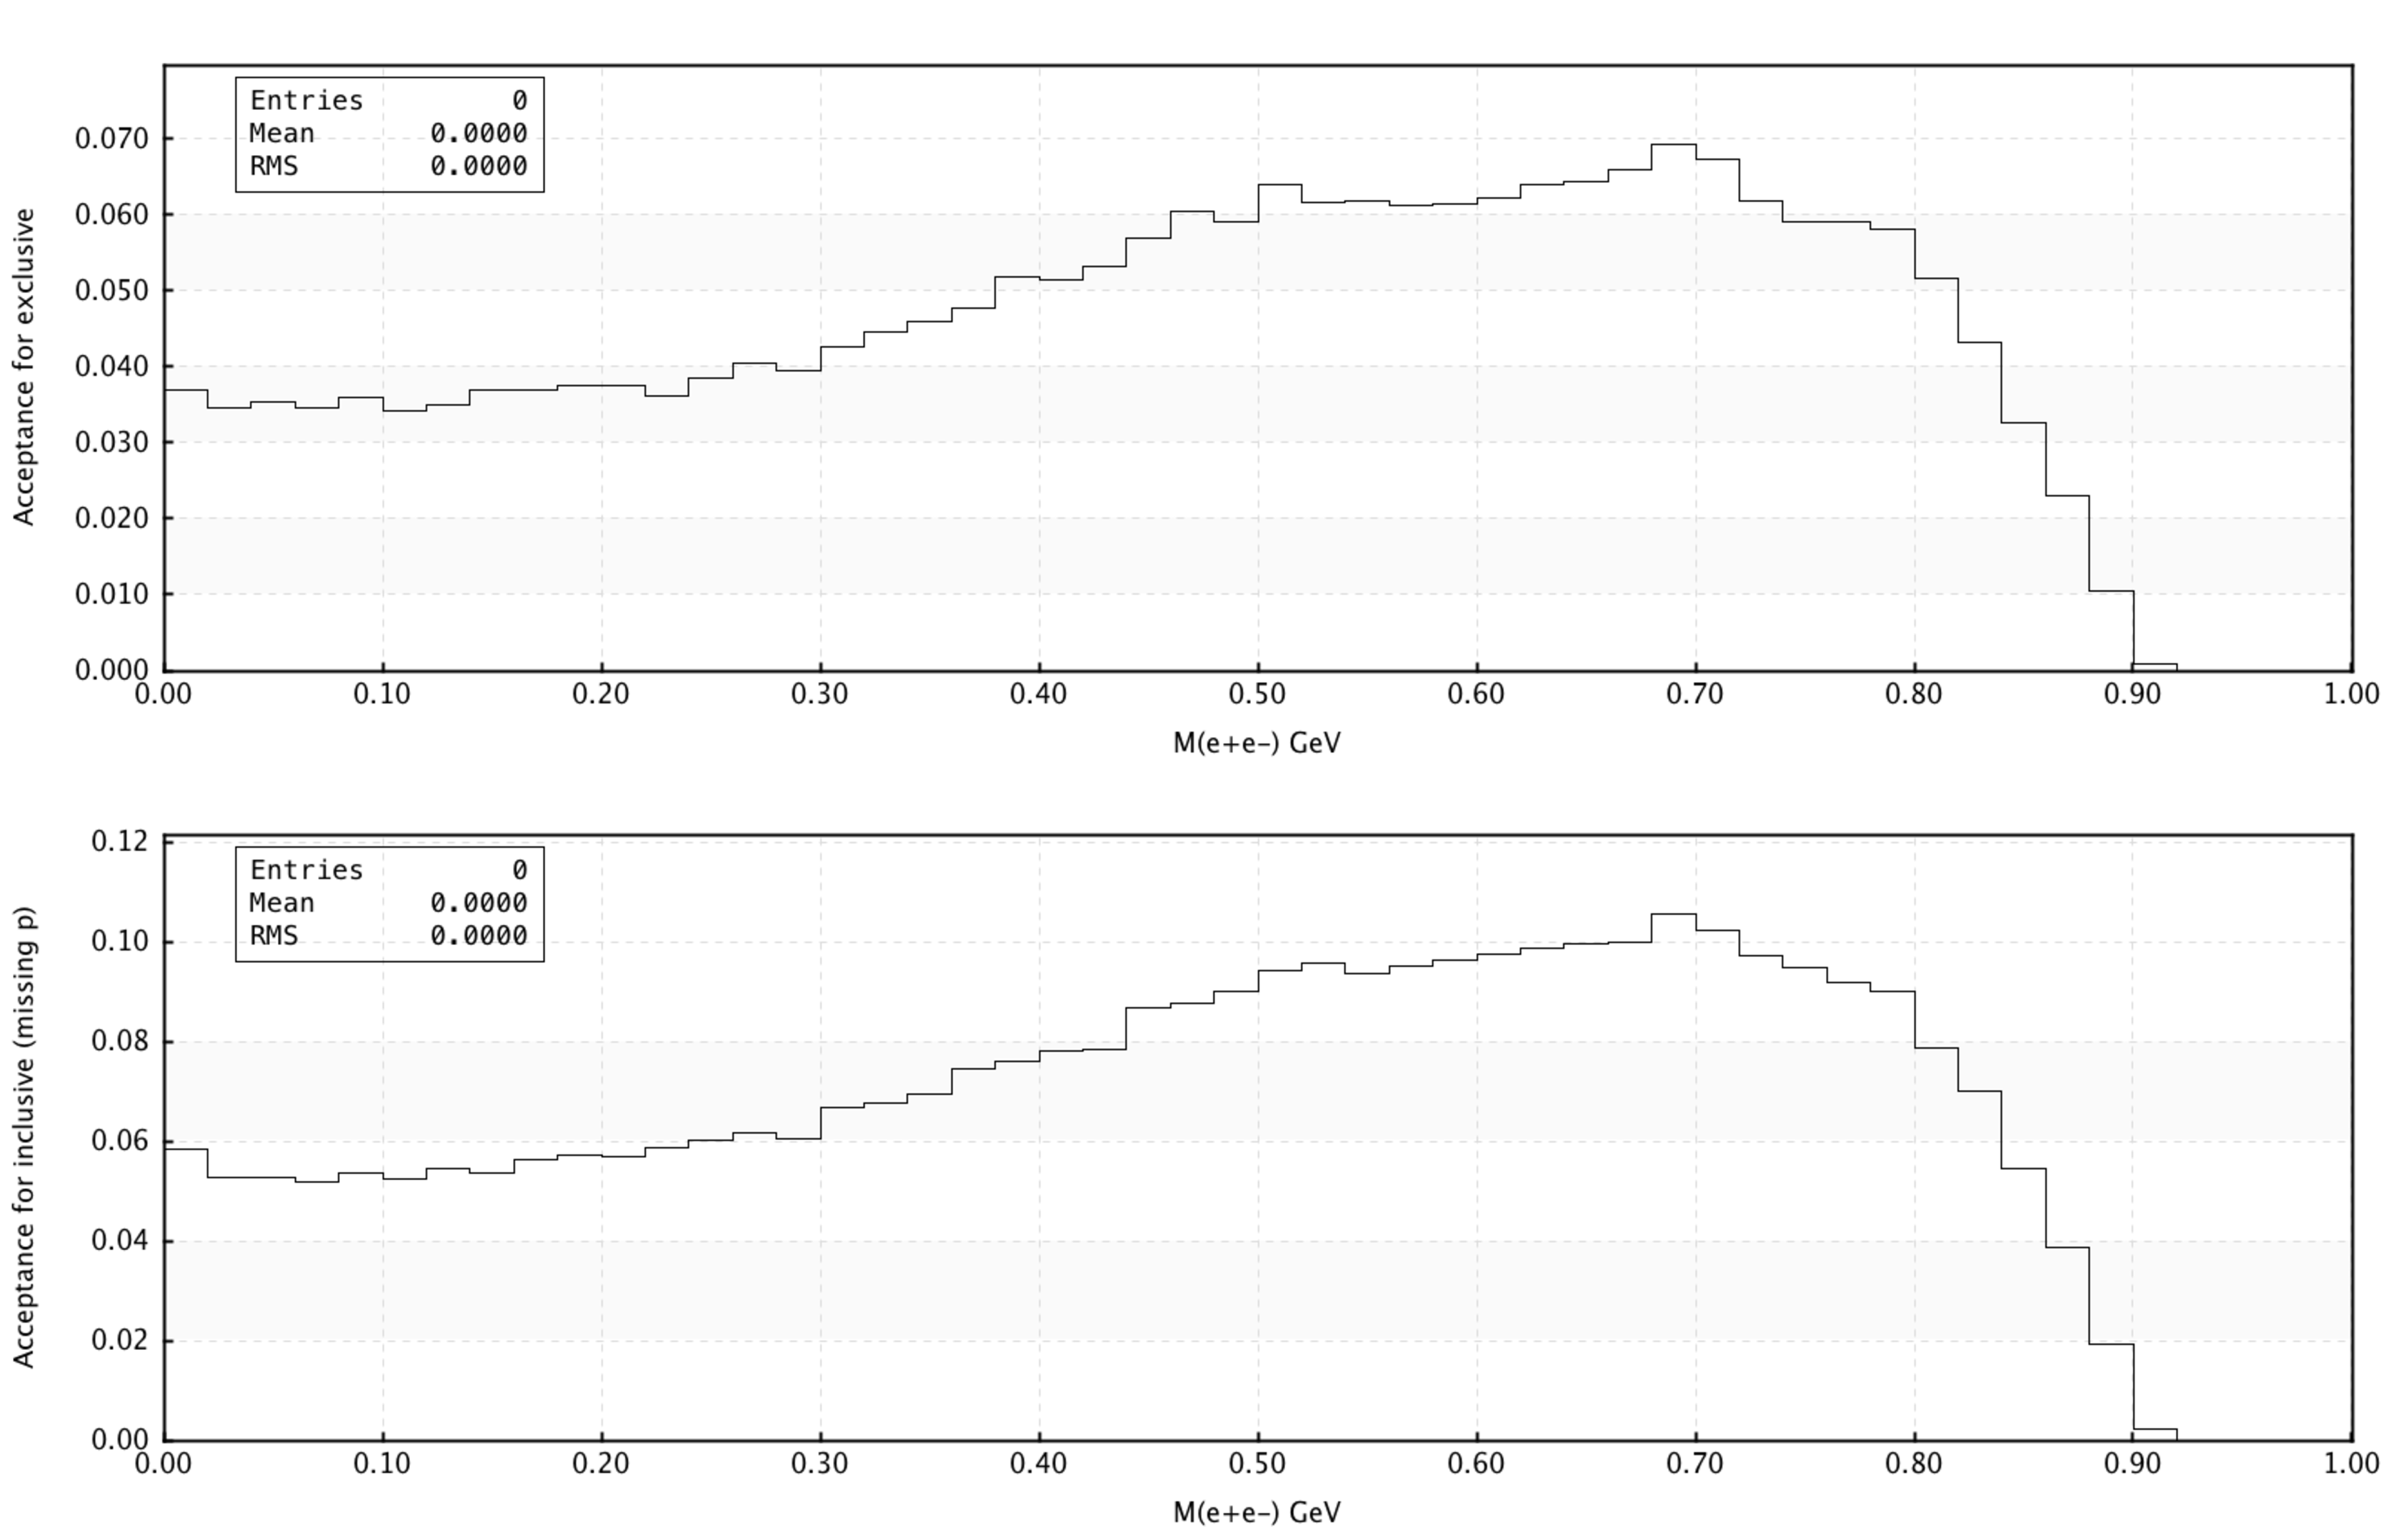
\includegraphics[width=\figwidth,height=1.2\qfigheight]{\grpath/counts/75_TORUS/FLAT/FLAT_Acceptance.pdf}
 		\caption[Acceptance, as a function of $M(\epem)$]{\label{fig:FLATaccepted}{Acceptance using a flat \epemT \ decay model, as a function of $M(\epem)$ for the exclusive (Top) and inclusive reconstruction scheme(Bottom).}}
 \end{center}\end{figure} 
\FloatBarrier




%%%%%%%%%%%%%%%%%%%%%%%%%%%%%%%%%%%%%%%
%THIS IS WHAT I ADDED:

\subsection{Calculating the Expected Yield}\label{sec:yield}
%\subsubsection{Calculating Photon Flux}\label{sec:calflux}
%A simple method for calculating the photon flux in CLAS12 is as follows; Using the fact that g12 had a photon flux of $7\cdot 10^7 \ \mathrm{\gamma/s}$ on a Au radiator of $10^{-4} \chi_0$ an expected $\sim 4\cdot 10^9  \mathrm{\gamma/s}$ will be seen in CLAS12 at ${\cal L} = 10^{35}\mathrm{cm^{-2}s^{-1}}$ on a 5~cm $\ell H_2$ target which is $\sim 5.7\cdot 10^{-3} \chi_0$. This number has been independently confirmed in a previous CLAS proposal~\cite{clas.proposal.meson}.

The expected yield for $ep\to e'p \etaP [\etaP\rightarrow p e^+e^- \gamma ]$ is calculated under the assumption, that the $\etaP$ electro-production cross-section can be deduced from the $\etaP$ photo-production cross-section. A qualitative justification of this assumption may be found in Fig.~\ref{fig:EtaProdX}. The shape of the cross-section distributions for $ep\rightarrow e'p\eta$, shown in the top row of Fig.~\ref{fig:EtaProdX}, are comparable to the corresponding distribution for $\gamma p\rightarrow p\eta$, plotted in the bottom row of Fig.~\ref{fig:EtaProdX}. The major difference is related to the scaling rule of $1/Q^2$, i.e. the electro-production cross-section might be approximated by the photo-production cross-section by scaling down the latter one by $1/Q^2$.

\begin{figure}[htbp]\begin{center}
		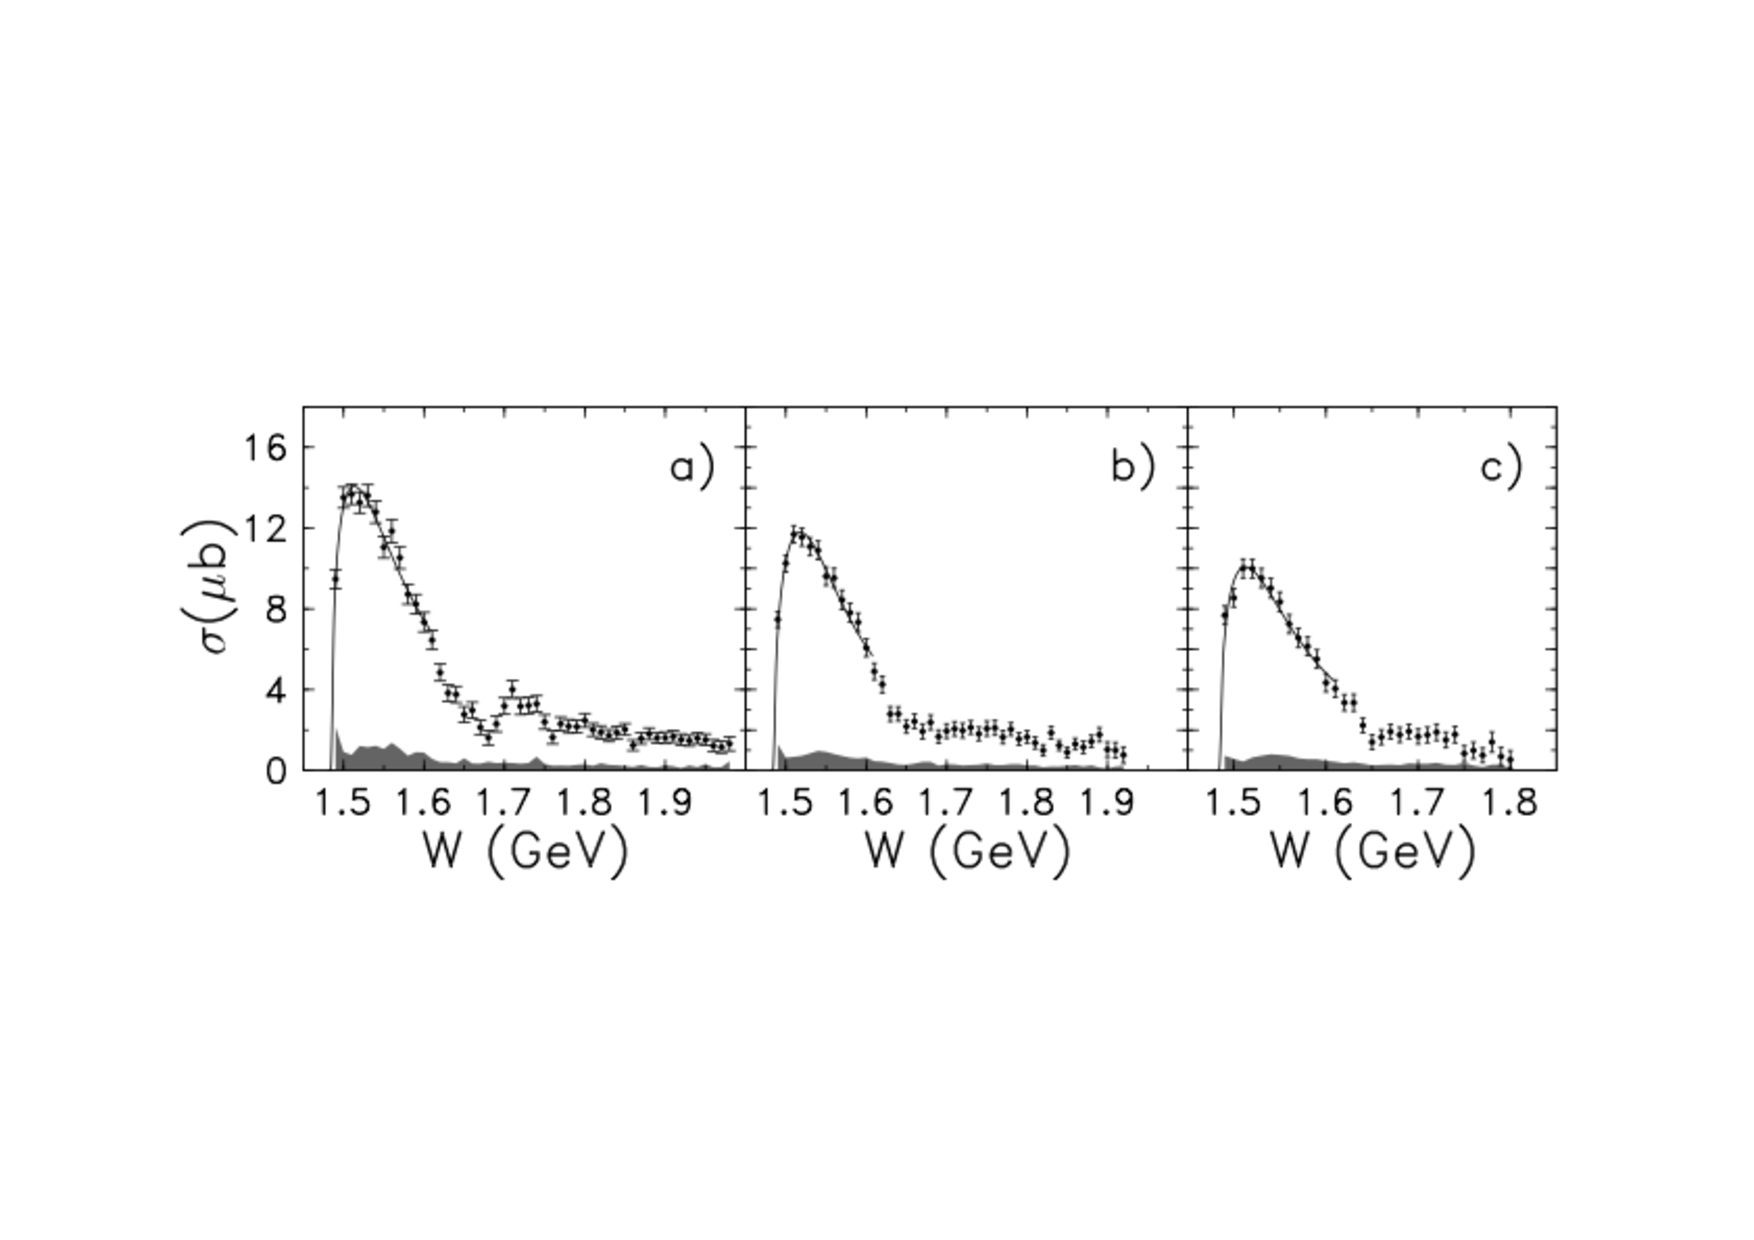
\includegraphics[width=\figwidth,height=1.2\qfigheight]{\grpath/XSection/eta_phot_electXSection.pdf}\\
		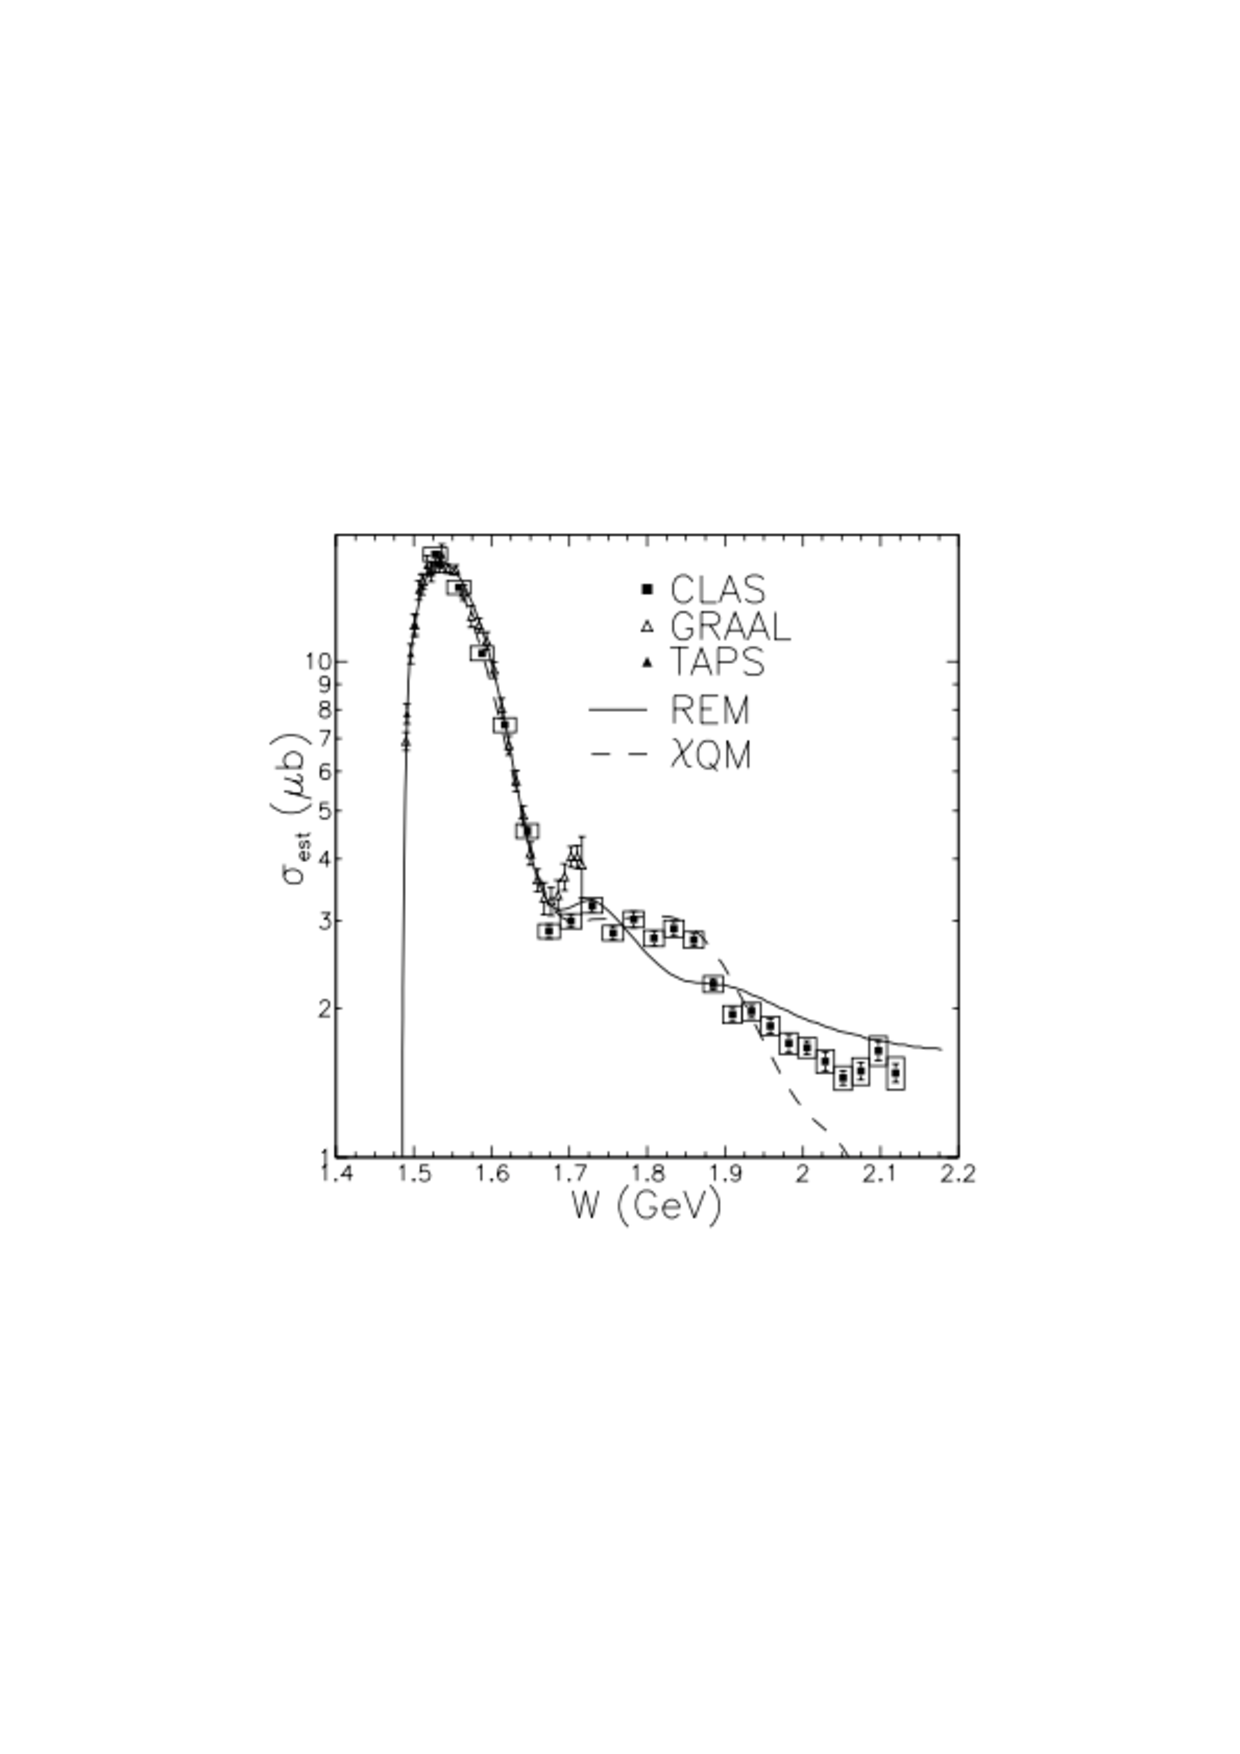
\includegraphics[width=0.7\figwidth,height=0.9\qfigheight]{\grpath/XSection/eta_phot_prodXSection.pdf}
		\caption[eta el-prod. XSection]{\label{fig:EtaProdX}{Integrated cross-section for $ep\to e'p\eta$ (Top) for: (a) $Q^2=0.625(GeV/c)^2$, (b) $Q^2=0.875(GeV/c)^2$, (a) $Q^2=1.125(GeV/c)^2$~\cite{etaelect} and for $\gamma p\rightarrow p\eta$ (Bottom)~\cite{etaphoto}.}}
\end{center}\end{figure}

\FloatBarrier

The top row of Fig.~\ref{fig:EtaPProdX} shows the total photo-production cross-section for hadrons in comparison with the photo-production cross-section for $\etaP$ (see bottom row of Fig.~\ref{fig:EtaPProdX}). Due to the considerations made above, these two cross-section distributions might be directly translated to the corresponding electro-production cross-sections. Using the distributions shown in Fig.~\ref{fig:EtaPProdX}, one might define the following ratio $R(W)$:

\begin{equation}
 R(W) = \frac{\sigma(W)}{\etaP\text{ integrated } \sigma(W)}
\label{XsecR}
\end{equation}

\begin{figure}[h!]\begin{center}
		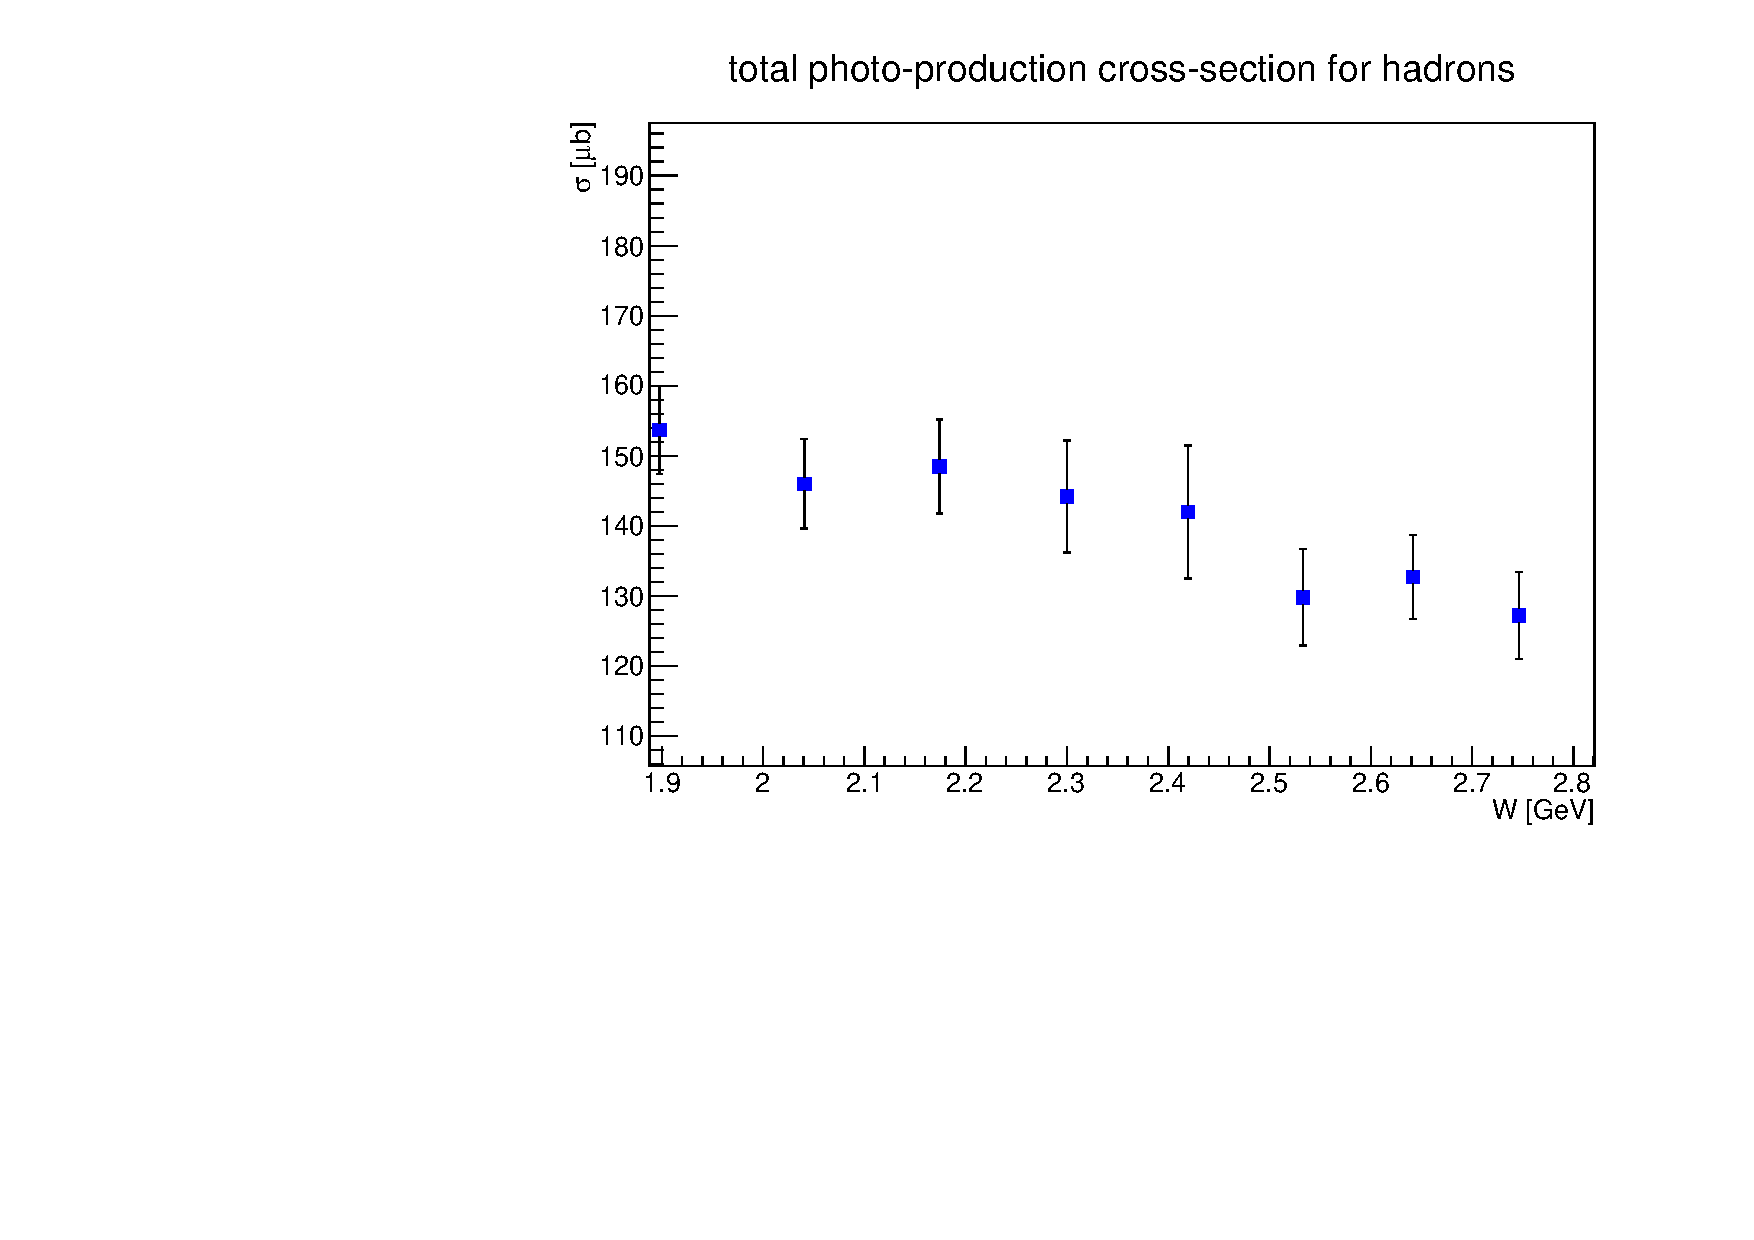
\includegraphics[width=0.9\figwidth,height=0.9\qfigheight]{\grpath/XSection/hadron_prod_photoproduction.pdf}\\
		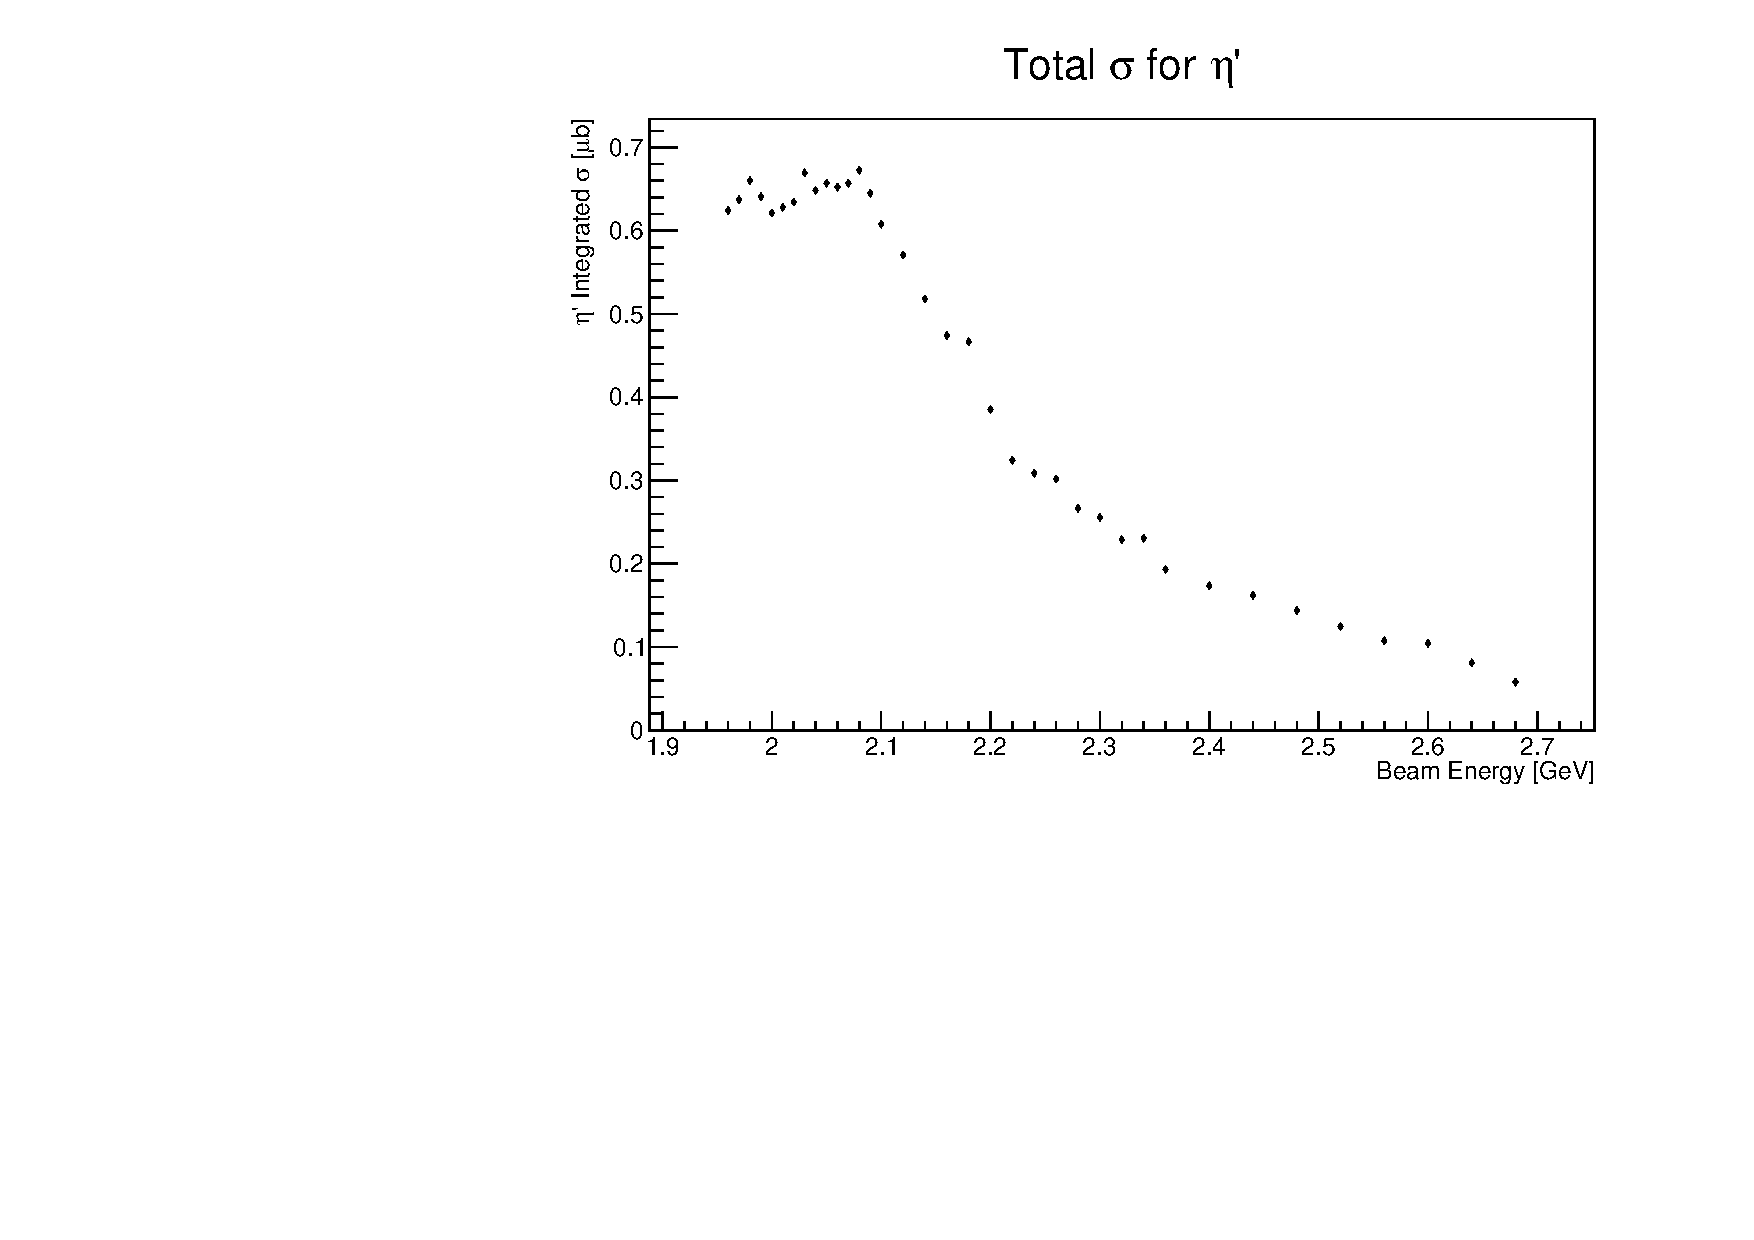
\includegraphics[width=0.9\figwidth,height=0.9\qfigheight]{\grpath/XSection/etaP_total_XSection.pdf}
		\caption[etaP phot-prod. XSection]{\label{fig:EtaPProdX}{Integrated cross-section for $\gamma p\rightarrow pX$ (Top) and $\gamma p\rightarrow p\etaP$ (Bottom) as a function of $W$.}}
\end{center}\end{figure}

The rate for mesons in electro-production where the scattered electron is left undetected is $\sim 140\,\rm{kHz}$~\cite{Sargsyan}. This rate needs to be scaled down by $R(W)$ in order to achieve the corresponding rate for $\etaP$ production. This leads to:

\begin{equation}
 \etaP\text{ total rates / 80 Days }(W) = 140\,\rm{kHz}\cdot \frac{86,400\mathrm{\ seconds}}{\text{80 days}}\cdot \frac{1}{R(W)}
\label{etaPRate}
\end{equation}

A plot of Eq.~\ref{etaPRate} is shown in Fig.~\ref{fig:EtaPRate} (left y-axis). The total $\etaP\rightarrow\epem\gamma$ rates per 80 days, and as a function $W$, is calculated by multiplying Eq.\ref{etaPRate} with the product of the average detection efficiency $\epsilon\approx 5\%$ as well as the branching fraction $\mathcal{BR} $ for $\etaP\rightarrow\epem\gamma$. The corresponding plot is shown in Fig.~\ref{fig:EtaPRate} (right y-axis). Obviously, the total number $N_{tot}$ of expected $\etaP\rightarrow\epem\gamma$ events after 80 days of measurement is given by the integral of Fig.~\ref{fig:EtaPRate} over $W$. This leads to the expected yield:

\begin{equation}
  N_{tot} = \int\limits_{1.9\,\rm{GeV}}^{2.8\,\rm{GeV}} \Big[ {\color{red}{N(W)_{\etaP\rightarrow\epem\gamma\text{ / 80 Days }}}} \Big]dW = \mathrm{\frac{52,100 \ events}{80 Days}}
\label{yield}
\end{equation}


\begin{figure}[h!]\begin{center}
		\includegraphics[width=0.9\figwidth,height=0.9\qfigheight]{\grpath/XSection/Total_rates.pdf}\\
		\caption[etaP rates]{\label{fig:EtaPRate}{Total $\etaP$ production rate per 80 days (left y-axis) and total $\etaP\rightarrow \epem\gamma$ rates per 80 days (right y-axis) as a function of $W$. Both rates have been calculated according to Eq.~\ref{etaPRate}}}
\end{center}\end{figure}


%%%%%%%%%%%%%%%%%%%%%%%%%%%%%%%%%%%%%%%





%\subsubsection{Expected Results}
%To extrapolate the number of $\etaP$ \ produced in 
%\\
%The average number of $\mathrm{meson} \to \epem X$ expected in CLAS12 can be calculated as:
%\begin{align}
%\bar{N}(\epem)_{\mathrm{meson}  \to \epem X} = \Phi \epsilon(\epem)\bar{\sigma} \rho_{\ell_{H_2}}\ell_{target}N_A \frac{\Gamma_{\mathrm{tot}_\mathrm{meson} }}{\Gamma_{\mathrm{meson}  \to \epem X}}\ ,
%\end{align}
%where $\Phi$ is the photon flux estimated in Sec.~\ref{sec:calflux}, $\epsilon$ is the acceptance, $\bar{\sigma}$ is the total cross-section, $\rho_{\ell_{H_2}}$ is the atomic density of $\ell_{H_2}$, $\ell_{target}$ is the target length, $N_A$ is Avogadro's constant, and $\frac{\Gamma_{\mathrm{tot}_\mathrm{meson}}}{\Gamma_{\mathrm{meson} \to \epem X}}$ is the total branching fraction of the meson decaying into $\epem X$.
%Using the lepton acceptance shown is Sec.~\ref{sec.reconstruction} the average number of \etaTP \  per $M(\epem)$ can be seen in Fig.~\ref{fig:etayield}.
% \begin{figure}[h!]\begin{center}
% \subfloat[$\etaP$ Dalitz and conversion spectra][]{ %Feynman diagram of $\etaP$ two photon decay
%	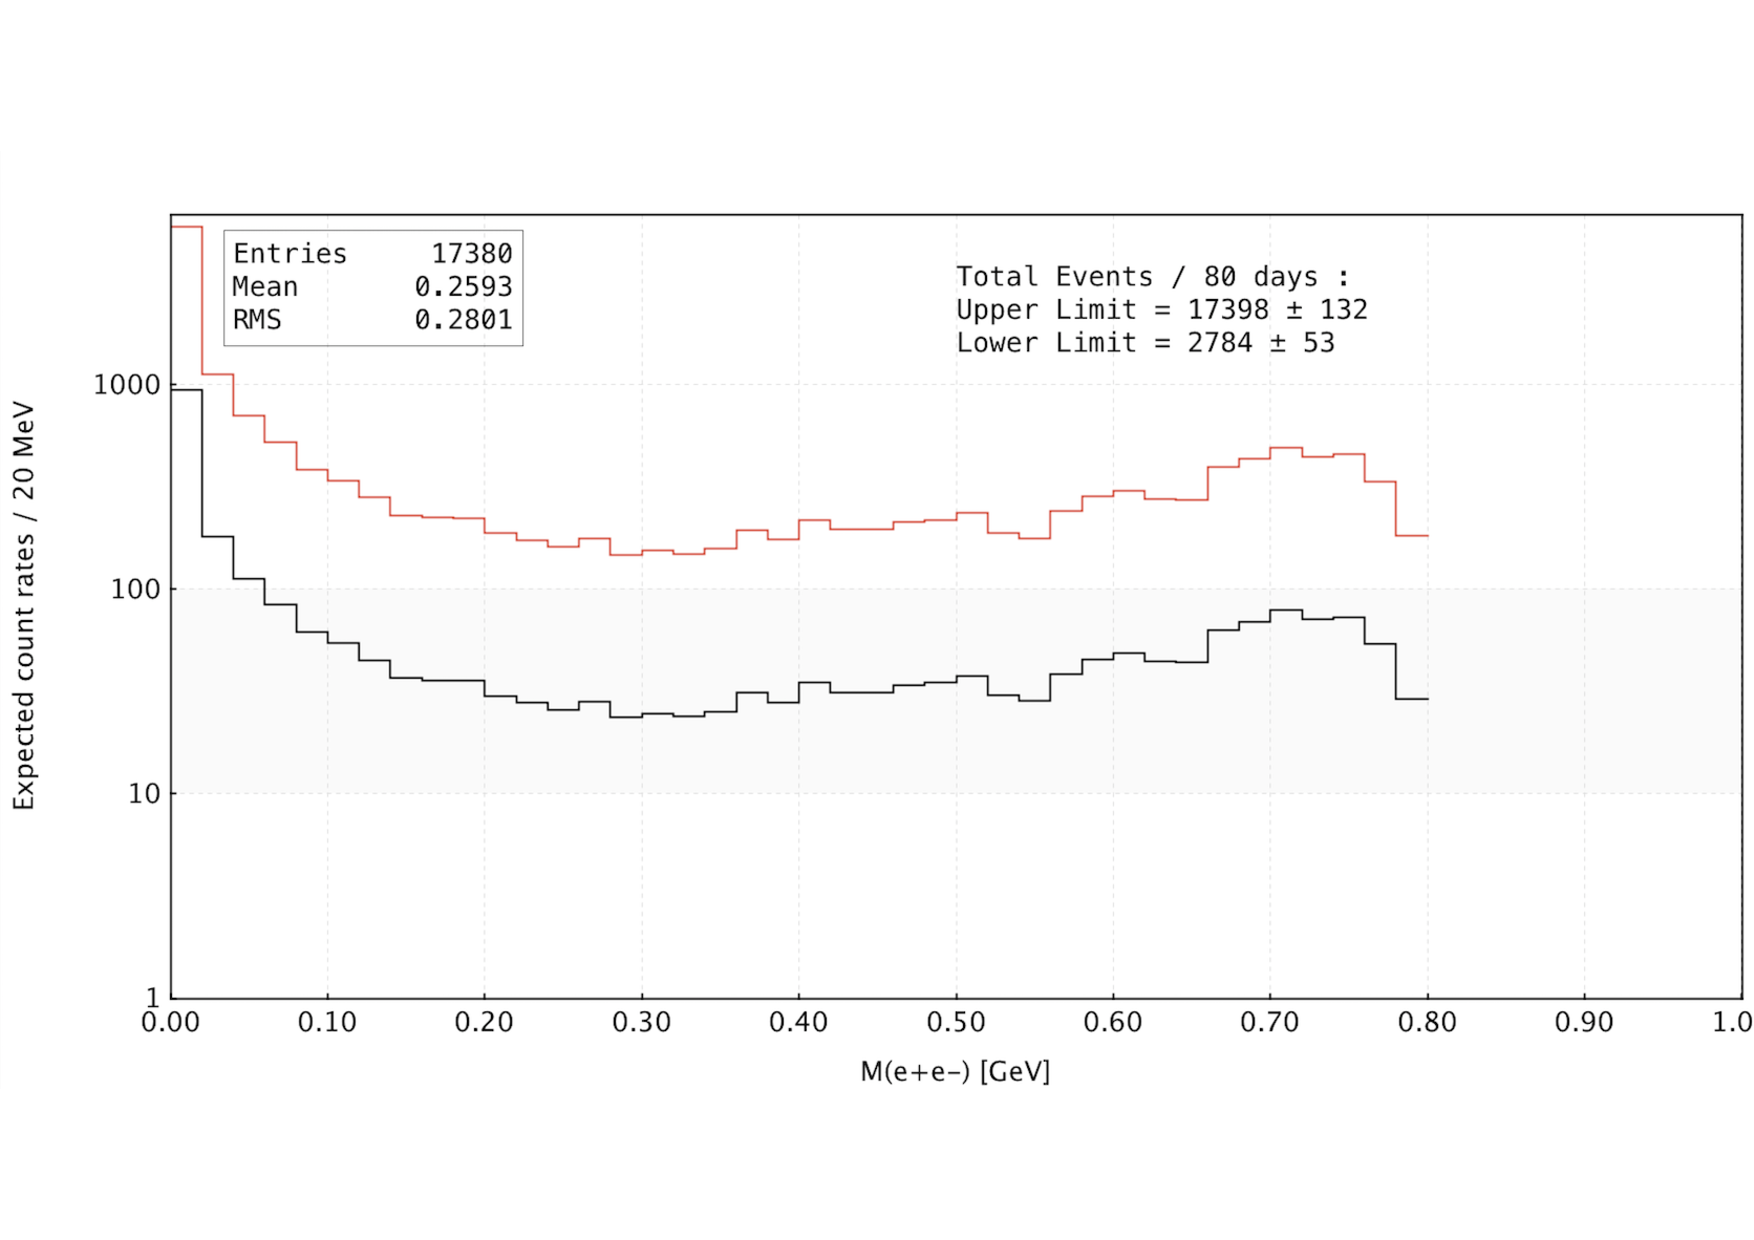
\includegraphics[width=0.8\columnwidth,height=1.0\qfigheight]{\grpath/counts/75_TORUS/VMD/VMD_Excluvise_count_rate.pdf}\label{fig:etap_count_exclu}
%	}
%\\
%\subfloat[$\phi$ Dalitz and conversion spectra][]{ %Feynman diagram of $\etaP$ Dalitz decay
%	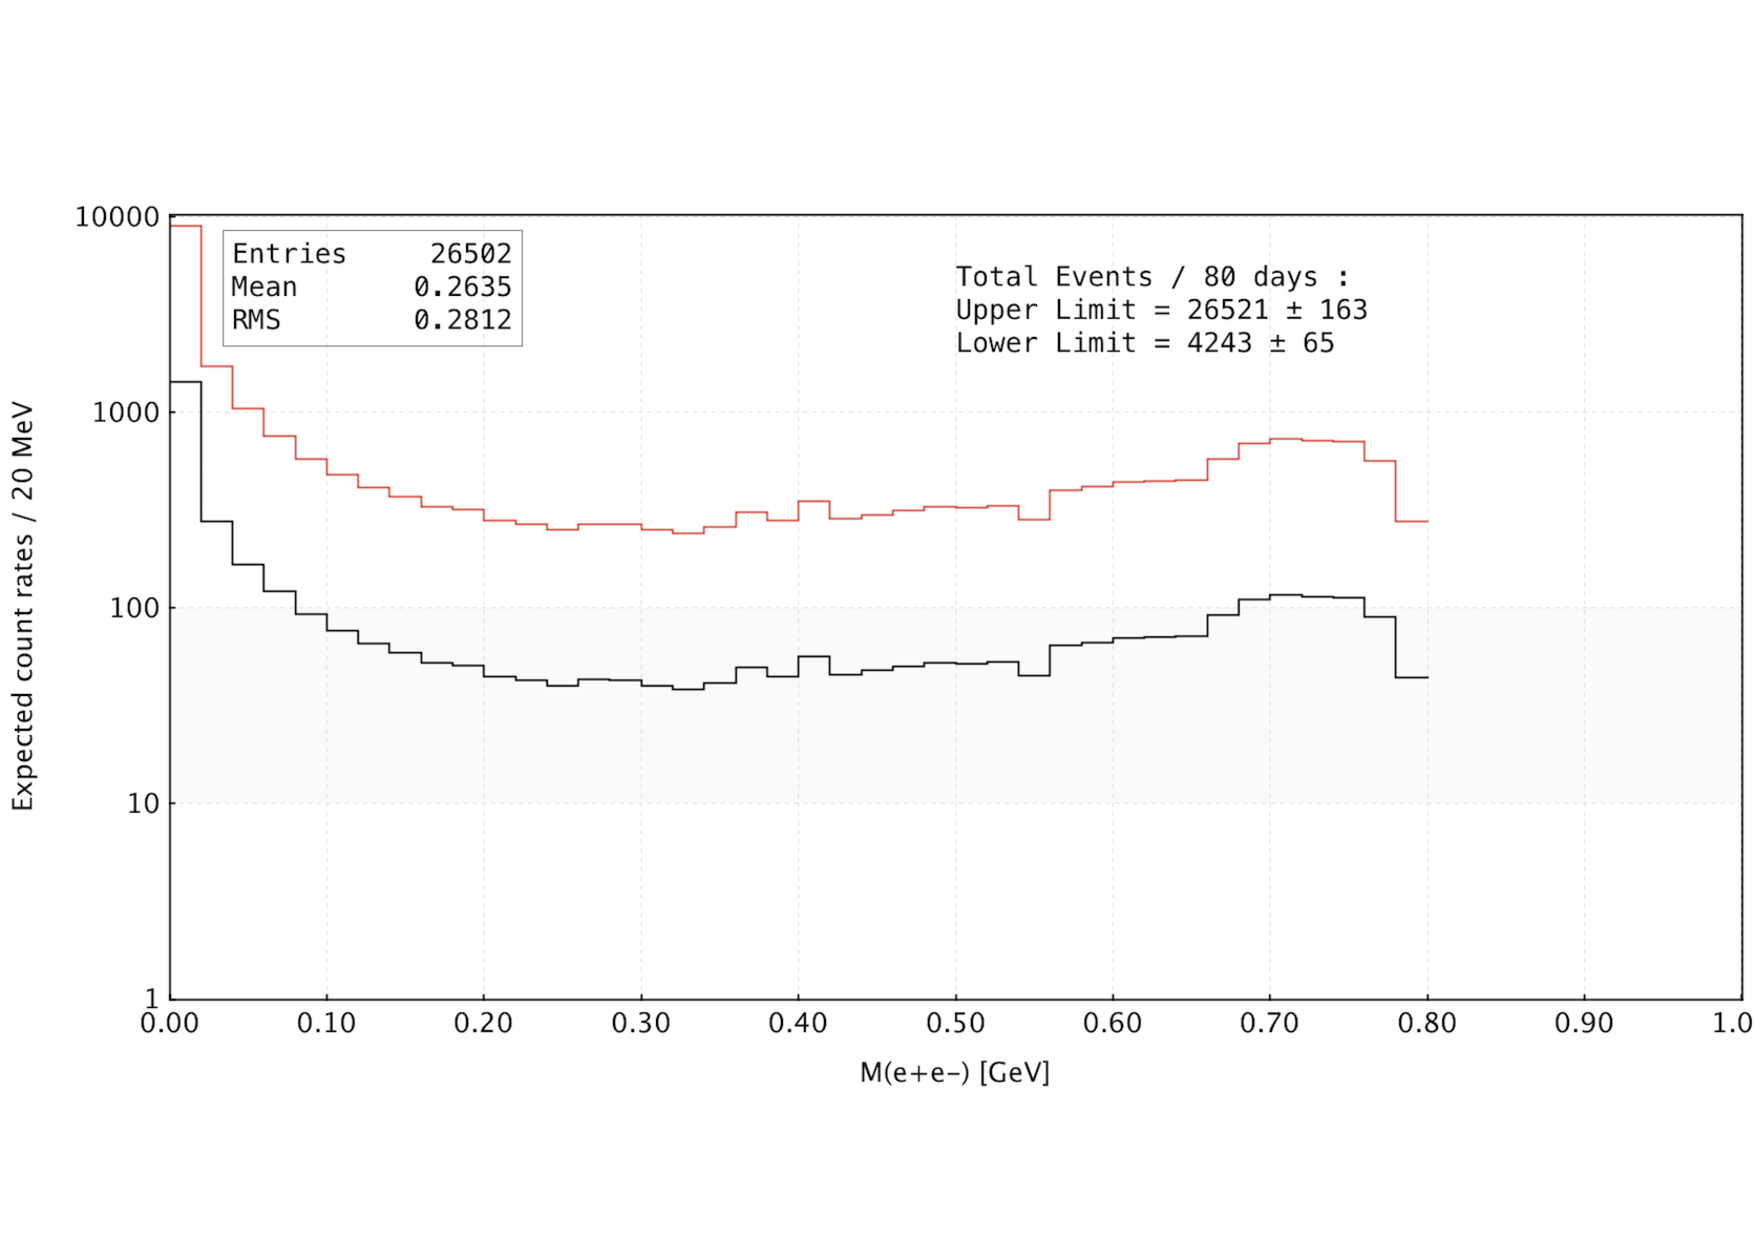
\includegraphics[width=0.8\columnwidth,height=1.0\qfigheight]{\grpath/counts/75_TORUS/VMD/VMD_Incluvise_count_rate.pdf}\label{fig:etap_count_inclu}
%	}
%\caption[Counts rates for \etaTP]{\label{fig:etayield}Count rates for the exclusive~\subref{fig:etap_count_exclu} and inclusive~\subref{fig:etap_count_inclu}. For both plots the photon detection efficiency was assumed to be between 10\%(Red) and  2\%(Black). }
%\end{center}\end{figure}
%\FloatBarrier
%Integrating over $M(\epem)$, the expected yield calculates to be $17,398$ events for exclusive scheme and $26,521$ events for the inclusive scheme. This would increase the world statistics by a factor of $\sim 20$ and $\sim 30$ respectively. 
%Table~\ref{tab:counts} and Tab.~\ref{tab:countsfull} in App.~\ref{sec:app.rates} depicts the upper and lower amount of \epemT expected from 80 days of beam time for two torus fields of 75\% and 100\% respectively.
%\FloatBarrier
%%\subsection{Realistic Yield}
%%As a reality check, lets compute the number of $\etaP \to \epem \gamma$ that g12 would have seen, had the experiment ran for 80 days with a real photon flux as calculated for CLAS12 (Sec.~\ref{sec:calflux}). %with the \epemT trigger configuration
%%The 89 $\etaP \to \epem \gamma$ events produced in g12 were recorded when the \epemT trigger was established. This time was 66\% of the total 44 days, which is $\sim29$ days. The total integrated flux measured during this time was $\sim 8.8\cdot 10^{13}$ photons. Therefore, in 80 days the total integrated flux would have been $\sim 2.4\cdot 10^{14}$ and the total number of \etaPDal \ events recorded would have been 242. The ratio of g12 total flux at 80 days per CLAS12 real photon flux is $2.73\cdot 10^{16} / 2.4\cdot 10^{14} \sim 114 $. Therefore g12 would have recorded $114\cdot 242 = 27590$ \etaPDal \ events, which is consistent with what is proposed to be measured with 80days, in the inclusive reconstruction scheme for either torus field setting. See Sec.~\ref{sec:app.rates} for total count rates.
\subsection{Acceptance at 100\% Torus field}
An addition simulation was performed using the same generated data shown above, the difference being the setting of the torus magnetic field. Below, in Fig.~\ref{fig:ratio}, the ratio of the lepton acceptance for the two different torus settings is depicted.
\begin{figure}[h!]\begin{center}
 		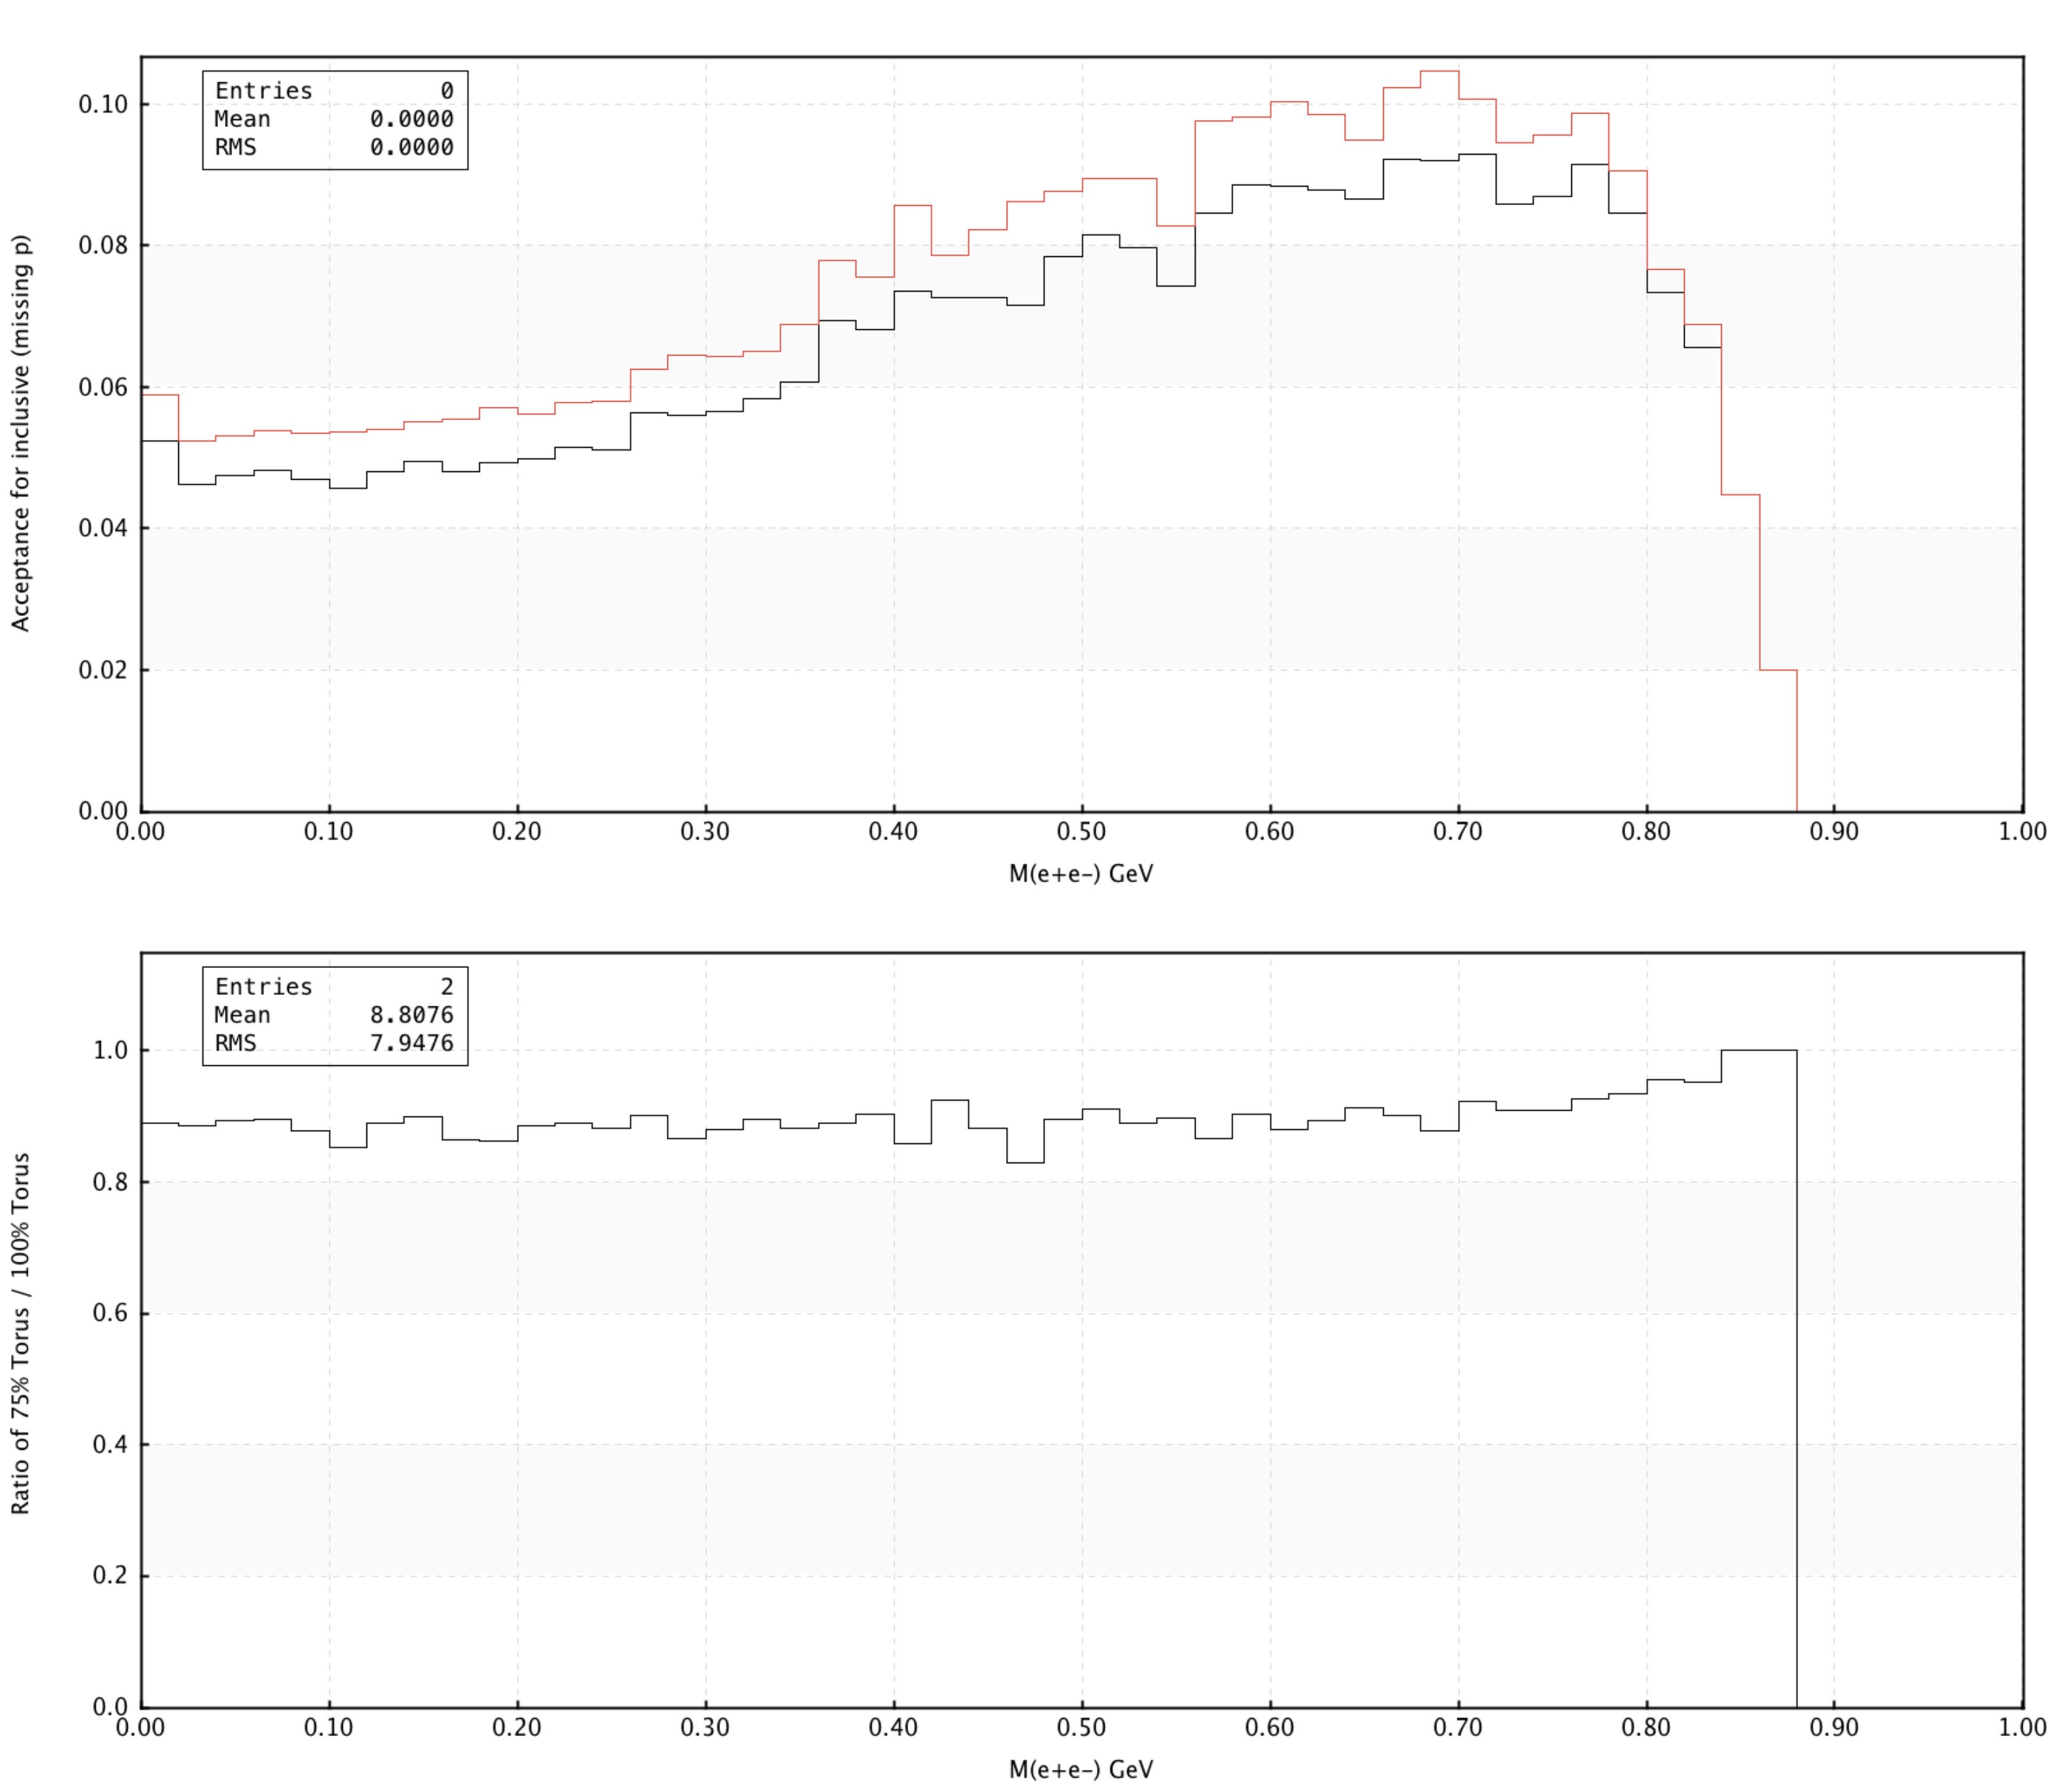
\includegraphics[width=\figwidth,height=1.6\qfigheight]{\grpath/counts/Ratio.pdf}
 		\caption[Acceptance, as a function of $M(\epem)$]{\label{fig:ratio}{Acceptance using a VMD decay model, as a function of $M(\epem)$ for the inclusive scheme(Top). The torus field was set to 75\%(red) as well as 100\%(black). Ratio of the acceptances plotted above (75\%/100\%)(Bottom). }}
\end{center}\end{figure}
\FloatBarrier
\subsection{Expected Systematic Uncertainties}
The major sources of systematic uncertainties are the acceptance and particle identification. The lepton acceptance uncertainty is estimated to be $\lesssim$ 5\% which was observed in former CLAS experiments. The lepton identification uncertainty will arise from the performance of the HTCC, PCAL and EC. From simulation studies performed for this proposal, all leptons and final state photons are detected within the geometric space of the PCAL+EC with hit coincidences in both. Furthermore, all leptons, within a few percent, that were detected in the PCAL+EC were also detected in the HTCC. Further systematics from pion contamination are mitigated by the pion rejection factor described above. Systematics related to external photon conversion are minimal due to the  1~mm resolution of the primary vertex given by the Silicon Vertex Tracker (SVT) as shown in Sec~\ref{sec:intro.conversion}. Any Bethe-Heitler contributions are negligible when utilizing and exclusive meson reconstruction scheme.



